\documentclass[10pt,a4paper,twoside]{report}
\usepackage{graphicx}
\usepackage{url}
\usepackage{float}
\usepackage{microtype}
\usepackage[explicit]{titlesec}
\usepackage[titletoc]{appendix}
\usepackage{lipsum}
\usepackage[normalem]{ulem}
\usepackage[hidelinks]{hyperref}
\useunder{\uline}{\ul}{}
\usepackage[hmarginratio=1:1]{geometry}
\usepackage{tikz}
\usepackage{fourier}
\usepackage{mdframed}
\usepackage{epigraph}
\usepackage{pdfpages}
\usepackage[titletoc]{appendix}
\usepackage[nottoc,numbib]{tocbibind}
\usepackage[type={CC},modifier={by-sa},version={4.0}]{doclicense}
\usepgflibrary{qrr.shapes.openrectangle}

%set header and footer
\usepackage{fancyhdr}
\pagestyle{fancy}
\chead{octoDrone: Simulation and Deployment for Autonomous Drone Networks}
\lhead{}
\rhead{}
\renewcommand{\footrulewidth}{0.4pt}% Line at the footer visible
\cfoot{\thepage}

\fancypagestyle{plain}{%
  \fancyhf{}%
  \fancyfoot[C]{}%
  \renewcommand{\headrulewidth}{0pt}% Line at the header invisible
  \renewcommand{\footrulewidth}{0.4pt}% Line at the footer visible
  \cfoot{\thepage}
}

%set chapter heading colours
\definecolor{mybluei}{RGB}{0,173,239}
\definecolor{myblueii}{RGB}{63,200,244}
\definecolor{myblueiii}{RGB}{199,234,253}

%set chapter heading tikz style
\tikzset{
mynode/.style={
  rounded corners=30pt,
  shape=open rectangle,
  open rectangle fill=myblueii,
  open rectangle sides=#1,
  }
}

%set up reference links
\hypersetup{colorlinks=true,allcolors=blue}
\bibliographystyle{plain}
\usetikzlibrary{shapes.geometric, arrows, positioning}

%look for images in the image folder
\graphicspath{{img/}}

%use 1.5x line spacing
\linespread{1.5}

%set up the aside environment
\newenvironment{aside}
  {\begin{mdframed}[style=0,%
      leftline=false,rightline=false,leftmargin=2em,rightmargin=2em,%
          innerleftmargin=0pt,innerrightmargin=0pt,linewidth=0.75pt,%
      skipabove=7pt,skipbelow=7pt]\small}
  {\end{mdframed}}

\begin{document}

%use roman numbering for the front matter
\pagenumbering{roman}
\begin{titlepage}
\begin{center}

\textsc{\LARGE CS407 Group Report}\\[1.5cm]
\vspace{1.5cm}

\hrule
\vspace{0.2cm}
\textsc{\LARGE octoDrone: Simulation and Deployment for Autonomous Drone Networks}\\
\vspace{0.2cm}
\hrule

\vspace{1.5cm}
\noindent
\begin{minipage}{0.4\textwidth}
	\begin{flushleft} \large
		\emph{Authors:}\\
		Alex \textsc{Henson}, \\ Ben \textsc{De Ivey}, \\ Jonathan \textsc{Gibson}, \\ William \textsc{Seymour} 
	\end{flushleft}
\end{minipage}%
\begin{minipage}{0.4\textwidth}
	\begin{flushright} \large
		\emph{Supervisor:} \\
		Dr.~Arshad \textsc{Jhumka} \\
		\emph{Secondary Marker:} \\
		Dr.~ Andrzej \textsc{Murawski} 
	\end{flushright}
\end{minipage}
\vfill
\large Department of Computer Science\\
\large University of Warwick\\
\large Summer 2016\\
\vfill

\includegraphics[width=0.50\textwidth]{img/dcslogo.png}~\\[1cm]
\end{center}
\end{titlepage}

\newgeometry{hmarginratio=2:3}

\tableofcontents
\listoffigures
\listoftables

\abstract{Drones and quadcopters are becoming increasingly prevalent in modern society, leading to increased research and development in the field of mobile sensor networks. This project, octoDrone, aimed to create a high quality network simulator targeted at quadcopters, with the aim of being accessible to academics and students alike. Through a focus on being abstract, we have created an application which is powerful, expressive, and can be deployed to almost all currently available hardware. This ability to use the same code for simulations and deployments allows for accurate benchmarking and verification of drone programs.}

%switch back to arabic numbering
\pagenumbering{arabic}

%set the chapter headings
\titleformat{\chapter}[display]
  {\normalfont\huge\sffamily}
  {}
  {20pt}
  {%
  \begin{tikzpicture}[remember picture,overlay]
  \node[
    anchor=west,
    rectangle,
    minimum height=4cm,
    text width=\paperwidth+1in,
    xshift=-\the\dimexpr\oddsidemargin+2in\relax,
    outer sep=0pt,
    fill=myblueiii] (titlerect) {};
  \node[
    anchor=south west,
    xshift=4.5cm,
    text width=\textwidth] 
    at ([yshift=5pt]titlerect.south west) {\fontsize{30}{36}\selectfont#1};
  \node[
    mynode=nw,
    anchor=south east,
    fill=myblueii,
    inner xsep=1.5cm,
    outer sep=0pt,
    font=\color{white},
    minimum height=30pt] 
    at (current page.east|-titlerect.north)
     {\bfseries\MakeUppercase{\chaptertitlename}\ \thechapter};
  \end{tikzpicture}%
  }
\titlespacing*{\chapter}
  {0pt}{-20pt}{60pt}

\setlength\beforeepigraphskip{1.5\baselineskip}
\setlength\afterepigraphskip{2\baselineskip}
\setlength\epigraphwidth{6.8cm}
\setlength\epigraphrule{0pt}
\renewcommand\epigraphsize{\large}
\renewcommand\textflush{flushright}

\let\oldepigraph\epigraph \renewcommand\epigraph[2]{%
  \oldepigraph{\color{mybluei}\itshape #1}{#2}}
 
\chapter{Opening}
\epigraph{``Once you have tasted flight, you will forever walk the earth with your eyes turned skyward, for there you have been, and there you will always long to return'' - Leonardo da Vinci}

\section{Key Words}
Autonomous Drones, Sensor Networks, Network Simulation, Communications Routing, Quadcopters.

\section{License}
This work is licensed under the Creative Commons Attribution-ShareAlike 4.0 International License. This means that you are free to:

\begin{itemize}
	\item \textbf{Share} - Copy and redistribute the material in any medium or format.
	\item \textbf{Adapt} - Remix, transform, and build upon the material.
\end{itemize}

for any purpose (even commercially) under the following terms: 

\begin{itemize}
	\item \textbf{Attribution} -  You must give appropriate credit, provide a link to the license, and indicate if changes were made. You may do so in any reasonable manner, but not in any way that suggests the licensor endorses you or your use.
	\item \textbf{ShareAlike} - If you remix, transform, or build upon the material, you must distribute your contributions under the same license as the original.
	\item \textbf{No additional restrictions} - If you remix, transform, or build upon the material, you must distribute your contributions under the same license as the original.
\end{itemize}

\begin{figure}[H]
	\centering
	\doclicenseImage
\end{figure}

\section{Acknowledgements}
We would like to thank a few people in particular for helping us through the vast amount of research and development that was undertaken as part of this project. Our project supervisor Arshad Jhumka has helped guide us, and the advice he gave us when we were considering changing the direction of the project was invaluable. In addition, campus security were very understanding when asked to retrieve one of the drones used for testing from the roof of the maths building, and spared us what could have been a lot of embarrassment and trouble. On a lighter note, we would also like to thank USB Man and Will's rubber duck, who both made development immeasurably smoother.

\section{Introduction}
Drones have exploded into the public conciousness in recent years, for reasons both bad and good. With companies such as Amazon using drones for delivery, and many studios using them for filming, it is clear that they will become and remain a part of everyday life. Research into networks of drones is still young, and requires a specific set of tools. This project aims to create a new application for simulating drone networks to aid both academic progress and outreach. With a focus on adaptability, it is hoped that octoDrone can be used as a domain specific testing tool which is generic enough to be deployable to most types of consumer and commercial hardware available.

This report will provide a comprehensive analysis of the project undertaken by our group. There will be a background summary of the key components in this field, as well as a discussion of the ongoing research, development, and production being carried out. An analysis of the potential problems for which a solution can be found in drone networks will be supplied, and justification given for the resulting aims and objectives of our group. The report will detail the design, implementation, and testing of the solution, including considerations for the management of the project. Finally, the project outcome will be evaluated, followed by a conclusion reflecting on the success of the project and considerations for future works.

\chapter{Background}
	\lettrine[lines=2]{T}{his} section will introduce the components which will be researched into that form the basis of the project. The aim of this section is to provide the reader with definitions for keywords which will appear on numerous occasions throughout the project, as well as helping to lead into a definition of the problem space and the objectives of the project as a result. 
	\section{Drones}
		\subsection{Definition}
		Unmanned Aerial Vehicles (UAVs), also known as drones, are aircraft which are either ‘piloted’, or perform autonomously using pre-programmed flight path and objectives \cite{chriscolejimwright2010}. Consumer-level drones are typically small in size, and take the form of quadcopters, which are multi-rotor helicopters with four rotors.  These types of drones are very lightweight, and powered by batteries; power consumption is almost completely attributed to fight time, although a modified drone will be required to exhaust power on its additional parts. We will be focusing on the use of these drones for the scale of this project.
		\subsection{Sensor Capabilities}
		Drones are typically equipped with cameras, as well as additional sensors, which vary depending on the type of drone, or its purpose. In the case of military drones, sensors such as multi-spectral targeting systems, night vision, infrared imaging and GPS are an absolute must \cite{usairforce2015}. However, mounted weaponry may also be included for direct warfare, unless the drone is designed specifically for intelligence, surveillance or reconnaissance, as power consumption is a primary concern, and must be limited. Military drones are controlled via satellite from a military base, although drones may also be controlled by Wi-Fi, radio or remote. Consumer-level drones have a wide range of usages, and the sensors that they require to accommodate these tasks are largely dependent on the price. It is possible to attach a large multitude of different sensors to drones; however the primary function of an aerial (consumer-level) drone is to collect high-quality imagery, often beyond the level of detail that the human eye can process.  These types of sensors include stereoscopic, thermal imaging, near-infrared and infrared, but other sensors such as thermal sensors and proximity sensors may also be used \cite{ questuav2015}.
		\subsection{Usages}
		Consumer-level drones have become increasingly popular in the past few years as they have become more affordable, capable and reliable to use. Due to their ability to capture high-quality imagery from impossible-to-reach locations, drones are incredibly useful in areas such as real estate, to take aerial shots of properties, or as a cheap alternative to huge, expensive helicopters for capturing news, such as high speed chases \cite{josephdussault2014}. Drones can also be employed for services such as delivery; there have been several initiatives for drone-based delivery of food or packaged goods by famous companies such as Amazon and Domino's Pizza \cite{marcusfaires2015}. Another possible usage for drones is in emergency services, such as the detection of forest fires, or search and rescue. It is these areas of drone research and development which can be considered to display the strength and importance of drones, as they are able to perform dangerous tasks which humans are incapable of and/or with no physical risk to human beings themselves. Compared to other types of mobile sensing, drones offer direct control over where to sample the environment, such that they can be explicitly told where to move to.
	\section{Sensor Networks}
		\subsection{Definition}
		A wireless sensor network (WSN) is a wireless network consisting of spatially distributed autonomous devices using sensors to monitor physical or environmental conditions. These devices are referred to as nodes, which are able to communicate with each other and with a base node, commonly referred to as a gateway, which provides connectivity between itself, the nodes and the rest of the wired world \cite{ nationalinstruments2012}. Nodes may vary in size and number depending on the network, but will typically contain transceivers, a battery, an electronic circuit for interfacing with sensors and an energy source.  The ability to cooperatively pass sensor data to a main location has implications in many different industries, as well as military applications.
		\subsection{Drone Networks}
		In the context of drones, this refers to a wirelessly connected network of autonomous drones with a base station, which can distribute information or commands to the drones in the network, as well as facilitate communication between them and itself.  Given that autonomous drones are emerging as a powerful new breed of mobile sensing system which can carry rich sensor payloads with various methods of control, a collaborative network of drones has considerable potential, and can greatly extend the capabilities of traditional sensing systems \cite{lucamottola2014}. 
	\section{Network Simulation}
		\subsection{Definition}
		As the name suggests, network simulation is a technique for modelling the behaviour of a network without performing a real, physical deployment, in order to test the effectiveness of the network, and assess how the network will behave under different conditions. Therefore, a simulation refers to software that predicts the behaviour of a network, so that performance can be analysed. By emulating an existing network, unexpected problems can be addressed or prevented prior to the deployment of the network.
		\subsection{Structure and Testing}
		A network simulation typically produces output in a GUI such that aspects of the network can be interpreted visually, such as to see how nodes interact, how data is sent, where connections go out of range or experience interference; it is possible to study the actual performance of a network and its protocols against the conceptual design. The simulation must be careful to provide an adequate level of detail to test the network without affecting the performance \cite{ leebreslauetal2000}. 
	\section{Routing}
		\subsection{Physical Routing}
		In order for mobile sensor networks to gather data about the environment, they will be required to navigate freely using predetermined pathfinding algorithms. For a drone network, a drone will be required to navigate 3-D airspace and collect sensing information, whilst being careful to maintain an efficient route and avoiding problems such as collision with its neighbours or the limitations of its physical components, such as battery life. Pathfinding must take into account the possibility of nonlinear dynamics, various constraints and changing environments \cite{robertsivillietal2012}.
		\subsection{Communications Routing}
		One of the core aspects of a sensor network is the ability for nodes to communicate with each other, relaying data back to the gateway. For an optimal routing algorithm, the exchange of data must be robust, avoiding congestion and maintaining connectivity when faced with mobility, whilst trying to maximise the duration for which the sensing task can be performed \cite{ curtschurgers2010}. The properties of communications routing which are to be optimised are dependent upon the type of sensor network; a drone network with less than thirty minutes of battery life must be optimised for energy consumption.

\chapter{Specification}
	\emph{In this section of the report, there will be an introduction to the problem space which is solvable using consumer-level drone networks (as defined in the previous section). After describing the problem, the objectives which need to be achieved in order to provide a solution for the problem space will be clearly laid out, as a means of outlining the foundation of the project. Justification for why the project solution to the aforementioned problem is both necessary and valid will also be given. There will be an analysis of the stakeholders in the project, followed by a feasibility study where a brief discussion of the scope of the problem which is to be handled will be provided, including the level of depth with which drone networks will be explored and implemented throughout the project.}

\emph{This study also allows us to identify the possible problems which may arise throughout the project and analyse its economic implications, as well as give a brief introduction to the management of the project. In doing so, it can be shown that the project is actually feasible to complete with the time and resources available. Having defined the objectives which must be completed to provide a solution for the project, the subsequent functional and non-functional requirements must be identified to ensure that the project deliverables are measurable and well-defined. Finally, any changes from the original specification at the beginning of the project will be briefly discussed, with justification for these changes.}

\section{Description of the Problem}
The problem, in the context of this project, is that there are many situations in which a drone sensor network could be well implemented to effectively carry out a task, but there is a lack of an environment for testing before going through the costly process of deployment. Simulators exist for the task of modelling sensor networks, but a generic network simulator does not exist which can be readily adapted to various hardware for use in multiple projects. For this project, the group has decided to focus on the task of creating a simulator which can be used for both modelling a drone sensor network through virtual stimulations, and as a framework for the code which implements physical deployment on a real network. An arbitrary problem for user tasking can be defined later which is impossible or risky for humans such as search and rescue, or high altitude photography, as well as problems which are feasible for humans, but can be more readily solved by UAVs, such as automated delivery. 

For this project, the objective that the group decided to focus on was the creation of a stimulator which would be built from first principles using the C++ programming language. Research into pre-existing network simulator libraries was performed in the literature review in section \ref{ns3design}. Considerations for the use of pre-existing network simulator libraries will be discussed in chapter \ref{ns3decision}, however it is sufficient to say that they were found to be difficult to tailor to the specific project requirements and the decision was made to focus on a project-specific solution of the group’s own design. The implementation of a simulator for a drone sensor network can hypothetically be applied to any similar problem area by altering the hardware arbitrarily (such as drone sensory inputs and outputs), which allows a solution to be provided for the general use case, and applied to various other situations.

The solution to this problem can be split into four main areas: the network simulation, the physical routing, the communications routing, and the physical deployment. In order to successfully create a solution to the problem described above, it is necessary to construct a stimulator which will accurately model the performance of the drone network, with associated physical and communications routing algorithms for optimal performance, before finally transferring this model to the physical drones and deploying them. The general solution can then be tested in a real situation, and then possibly extended to handle specific problem-solving tasks with user input such as the detection of forest fires. 
\section{Objectives}
\label{sec:obj}
The aim of this project, then, is to design and implement a general-use simulator for a drone sensor network in order to provide a generic solution to the problem of modelling sensor networks and the establishment of a framework for implementing physical deployment. This solution will provide the basis for research and extension into any potential situation in the field of drone sensor networks. The major components of the project were outlined in the initial project specification during the early stages of the project life cycle, and can be summarised as follows: 
\begin{enumerate}
  \item \textbf{Implement a network simulator}. Either using a pre-existing set of libraries, or by creating our own, which are specifically tailored to our domain.
  \item \textbf{Establish a network of drones with a base station}. Drones can communicate with one another and the base station, sending data between them.
  \item \textbf{Provide autonomy to drones}. Each drone must be able to dynamically control itself, as opposed to remote control, in order to operate autonomously in a network.
\item \textbf{Implement drone pathfinding}. Drones must carefully navigate through an area of physical space using well-defined rules for physical routing.
\item \textbf{User input tasking}. The user must be able to define a problem for the network to detect, which is passed from the base station to the drones.
\item \textbf{Implement problem detection}. Drones use sensory information to collect and pass data, notifying the base station in the event of a problem.
\end{enumerate}
These tasks have been scheduled using a Gantt chart which can be seen in \ref{gantt}, where tasks can be assigned to each group member based on their individual skills as necessary for maximum efficiency. Certain tasks, such as communication and pathfinding can be developed in parallel. Delegation of tasks and group roles will be discussed in depth in later sections.

\section{Justification}
The benefits of carrying out a project involved in creating an efficient, extensible solution to network simulators are relatively self-explanatory. The project is justifiable in its ability to produce a framework for extensive research and development in the field of sensor networks, with potentially life-saving results. Drone networks themselves are an area of research which is growing in popularity, so the project interacts well with the state-of-the-art and could have considerable impact on future developments. A general use solution based on the project software would be easy to use and deploy, and incredibly extensible.

\section{Stakeholder Analysis}
As previously discussed, the implementation of a drone sensor network has implications for a wide variety of industries. This section will therefore give a formal outline of the prospective stakeholders in the project and the justification for them. Firstly, given that drone sensor networks are a relatively new field of research, those parties interested in research and development of sensor networks would also benefit from the project. The results may extend the field of research, and the project solution could be adapted for use in other areas.  Example applications for indirect stakeholders could include detection and response to forest fires, emergency services such as firefighters, ambulance services, and search and rescue, who would benefit greatly by providing the ability to pre-empt danger and respond to crises much more rapidly, as well as reducing the risk to human lives in combating fires. In the same way, commercial businesses such as real estate and delivery services in pursuit of more efficient business may also benefit from the project. Finally, the project can be used for outreach, in terms of being educational, by teaching the concepts surrounding simulators and drone networks, as well as the algorithms which have been implemented in the code.

\section{Feasibility Study}
While the merits of the project are justifiable, it should also be noted that the project implementation carries a considerable technical difficulty.  Individual consumer-level drones must be adapted to programmable, autonomous drones which function as a sensor network capable of communications and pathfinding, which are to be simulated and then physically deployed. Therefore, it is important to analyse the feasibility of the project given time, hardware and other constraints, which will be discussed in the following sections.

\subsection{Problem Scope}
It is important to consider the scope of the problem, with regards to how far the solution can be extended into the domain of, in this case, network simulators. Given that drone sensor networks are a relatively new domain for research and development, there is no commonly used and accepted standard for drone networks in the context of network simulation. In other words, the solution to the problem is not an extension of a previously existing solution, or of a set of rules governing how the problem can and should be solved using drone sensor networks.

As a result, the scope must be carefully defined such that an effective solution can be reached for the problem without expanding too far into the problem domain. By implementing a drone sensor network which can be adopted into any general use case and can be easily extended to take any required sensory information and applied to solve a problem, the project avoids being overextended. At the same time, in order to show that the network can effectively handle user input tasking, one piece of sensor information was focused on, such as thermal, to demonstrate an accurate model for problem detection (as defined by the user) and response through well-established communications. 

\subsection{Project Scope}
Having defined the scope of the problem, it is also necessary to examine the scope of the project itself in terms of how far the project can extend into the domain of drone sensor networks. The implementation of any sensor network requires a lot of concise testing and a solid formation of protocols. There are many areas to consider with physical routing and communications, as well as physical deployment and use tasking. When creating the network simulator, it can be tailored to project-specific requirements in order to minimise the amount of considerations for network protocols and possible problems (discussed later), whilst accurately modelling physical deployment. 

Considering the time constraints that are imposed on the project, it will also be necessary to adapt pre-existing algorithms to establish our network communications and physical routing as opposed to creating our own algorithm, which would be suboptimal. In terms of physical deployment, the project is limited to two drones, so it is only possible to implement a minimum working example of a network to test the solution. Nonetheless, it is possible to show that the network is theoretically scalable and accurately demonstrates the ability for drones to communicate and use pathfinding effectively.

\subsection{Financial Analysis}
The basic requirements for a physical drone network are the drones themselves, the sensors which will be attached to the drones, as well as equipment for programming the drones and communications. All of these are provided by the Department, so financial constraints for physical deployment are limited to (a budget of) what the Department is able to provide. While it is possible to purchase more drones, the same result can be achieved, provided that at least two drones are available. Additionally, the project will not include the use of any bespoke software or libraries in the development of the simulator or communications; they will be open source, so there are no costs incurred in the development of the project.

\subsection{Market Analysis}
For the project to be used by third parties, there must be licensing associated with the final product. As the project is intended to be open source and not commercialised, the project software will be using the GNU General Public License v3.0, which stipulates that our project is open source, with the freedom to use or change the software, as well as distribute it and share changes. However, in the event that the project is used, the software creators are not accountable for any problems with the project software. As the project is not commercial, with no intention to monetise it, the use of this license allows us to appease any and all stakeholders whilst protecting ourselves from potential threats.

\subsection{Project Management}
There are many challenges associated with undertaking a project such as this, particularly with regards to administration, scheduling and the division of tasks. Therefore, it is crucial that the project is managed efficiently, and that progress is carefully monitored and assessed throughout the life-cycle of the project. The issues associated with project management and how they were handled throughout the project will be discussed later on in the project management chapter of the project. However, there are several challenges that the project group will be presented with in the context of project management, which are summarised below:
\begin{itemize}
\item \textbf{Development methodology}. There must be consideration for a development methodology which accommodates the size of the group and the time each group member has available, as well as how to track the progress of the project
\item \textbf{Deadlines and scheduling}. Meetings and deadlines must be scheduled such that the group is fully aware of what stage of the project must be completed and when. Interested parties such as the project supervisor must also be regularly informed of the progress of the project to allow for appropriate advisory actions where necessary
\item \textbf{Group roles}. Each member of the group must have a clear and distinct role in the group, with one member taking the role of project manager, dedicated to handling each group member and their associated tasks, as well as managing the state of the project to ensure that it is completed effectively and within constraints
\item \textbf{Managing project materials}. It is necessary to manage the project material to ensure consistency amongst each members’ work, as well as maintaining previous iterations of code to avoid problems such as losing previous functionality
\end{itemize}

\section{Requirements Identification}
This section will contain a list of the functional and non-functional requirements identified at the beginning of the project which will be necessary to implement to ensure that the project software adequately represents a solution to the problem as defined in this chapter. A functional requirement refers to quantitative requirements which can be easily measured and tested to ensure correct functionality. Non-functional requirements are those which cannot be measured, as they are subjective, but are nonetheless important for a successful project outcome. 

\subsection{Functional Requirements}
A list of the functional requirements for the project can be found in table \ref{functable}.
\begin{table}[]
\centering
\caption{List of functional requirements for the project software}
\label{functable}
\begin{tabular}{|l|l|}
\hline
\#  & Description                                                                                                                                                                                               \\ \hline
R1  & \begin{tabular}[c]{@{}l@{}}User must be able to run an executable which contains the\\   simulation environment and communications module\end{tabular}                                                    \\ \hline
R2  & \begin{tabular}[c]{@{}l@{}}A class must be instantiated for the nodes of the simulator (i.e.\\   drones and base station)  and a\\   communications module must be installed on each of them\end{tabular} \\ \hline
R3  & \begin{tabular}[c]{@{}l@{}}The simulation must run, such that each node begins to operate and\\   ‘travel’ within the environment\end{tabular}                                                            \\ \hline
R4  & \begin{tabular}[c]{@{}l@{}}Each node must be capable of sending, listening for and receiving\\   messages over Wi-Fi/radio\end{tabular}                                                                   \\ \hline
R5  & \begin{tabular}[c]{@{}l@{}}The environment must incorporate and handle multithreading for each\\   node\end{tabular}                                                                                      \\ \hline
R6  & \begin{tabular}[c]{@{}l@{}}The simulation must be able to model and be robust to interference\\   between message passing\end{tabular}                                                                    \\ \hline
R7  & \begin{tabular}[c]{@{}l@{}}The user must be able to see output from each node as messages are\\   sent and received\end{tabular}                                                                          \\ \hline
R8  & \begin{tabular}[c]{@{}l@{}}The user must be able to visualise the output of the simulation on a\\   graphical interface\end{tabular}                                                                      \\ \hline
R9  & \begin{tabular}[c]{@{}l@{}}The base station node must be able to take user input which can be\\   broadcast to other nodes\end{tabular}                                                                   \\ \hline
R10 & \begin{tabular}[c]{@{}l@{}}The simulation must be capable of communications from any\\   (preselected) algorithms\end{tabular}                                                                            \\ \hline
R11 & \begin{tabular}[c]{@{}l@{}}The environment and its respective nodes should stop running when a\\ command to do so (a message) is received\end{tabular}                                                    \\ \hline
R12 & \begin{tabular}[c]{@{}l@{}}Nodes must be capable of moving through the environment autonomously\\   using pathfinding algorithms\end{tabular}                                                             \\ \hline
R13 & \begin{tabular}[c]{@{}l@{}}Nodes must be able to recognise useful sensory information, and\\   broadcast the information back to the base station\end{tabular}                                            \\ \hline
R14 & \begin{tabular}[c]{@{}l@{}}The simulation code must be adaptable to the physical drones for real\\   deployment\end{tabular}                                                                              \\ \hline
\end{tabular}
\end{table}

\subsection{Non-functional Requirements}
A list of non-functional requirements can be found in table \ref{nonfunctab}.
\begin{table}[]
\centering
\caption{Table of non-functional requirements for the project}
\label{nonfunctab}
\begin{tabular}{|l|l|}
\hline
\# & Description                                                                                                            \\ \hline
R1 & \begin{tabular}[c]{@{}l@{}}Must follow existing simulator conventions so as to be easy to use by researchers\end{tabular}     \\ \hline
R2 & Simulation must be able to model interference accurately                                                      \\ \hline
R3 & \begin{tabular}[c]{@{}l@{}}Must be accessible to students with limited technical knowledge \end{tabular} \\ \hline
R4 & The user must be satisfied with the output from the environment                                                        \\ \hline
R5 & The final code must be extensible for more specific use cases                                                          \\ \hline 
\end{tabular}
\end{table}

\section{Project Deliverables}
Throughout the course of the project, there are several deadlines that must be met for which the project will be required to deliver a product. At the beginning of the project, the project specification was submitted in Term 1, which introduces the project and its initial planning and methodology, which will be appended to the report for reference. At the end of Term 1, a poster presentation was given by the project group to select supervisors and invigilators, and a live demo of the project software and this report will be delivered at the beginning of Term 3. The demo will display the proposed solution to the problem defined at the start of the project, and showcase the features of the working solution. Alongside this report, the code for the project, including the simulation, communications routing, physical routing and deployment code will also be submitted.

\section{Changes From Original Specification}
In the original specification, it was stated that ns-3, a set of network simulator libraries, would serve as the core implementation of the simulator, and that the code for physical deployment would then be built off of the simulator as a result. However, it was decided to instead build a simulator from scratch, after discovering that ns-3 is relatively bloated and difficult to use. The benefits to creating our own stimulator are that the code can then be directly translated onto the drones during deployment, as well as being directly tailored to the project domain. As a result, the functionality provided by ns-3 must be manually generated, which may increase the complexity of the project.


\chapter{Literature Review}
	\label{litreview}
\emph{This chapter of the report focuses on examination and analysis of current research and development in the field, in order to find out more about the structure of Mobile ad hoc networks (MANETs) and corresponding simulators, how drones can be employed in this field, as well as existing solutions for drone sensor networks. Then, the specific algorithms and characteristics of sensor networks must be researched, as this dictates the core functionality of the project network and how this can be achieved. This chapter will be cover the topics of learning about the current state-of-the-art, and allowing that to influence our design and implementation decisions.}

\section{MANETs}

\subsection{Structure}
It is necessary for a MANET to be capable of self-configuring without an infrastructure, where mobile devices can connect without wires. This is because mobile nodes communicate by forming a network dynamically, and so they lack a fixed infrastructure or centralised control. Nodes are independent, and the network topology is temporary as each node dynamically self-organises. This means that each device must be a router. Each node must be aware of the organisation when forwarding packets \cite{jaydipsen2010}. When nodes wish to communicate with one another they can use a variety of different mediums, such as Wi-Fi or radio waves, but they must depend on intermediate nodes to route their data packets in the event that the source and destination are not in range of one another \cite{ramramathanjasonredi2012}.
MANETs may employ a specific network model, or a general approach in which nodes are aware of other nodes in range and their task only. Various methods of forwarding data exist, such as flooding data by broadcasting to all neighbours, or by using predefined metrics to determine the optimal path \cite{jaydipsen2010}. It is in stark contrast to a centralised wireless network, as there are no access points in a managed infrastructure. Forwarding of data is dependent on the presence of network connectivity, so nodes must be able to create and join networks arbitrarily, which requires high adaptability to constant changes in topology. MANET systems must also consider problems such as limited power and storage for each individual node; the network must be fault tolerant such that it can deal with problems such as when connectivity is lost or a node powers down. Energy and power consumption are priority concerns which are directly related to the hardware resources available to each node, and the environment in which the network is deployed \cite{sajshahmina2012}.

\begin{figure}
\centering	
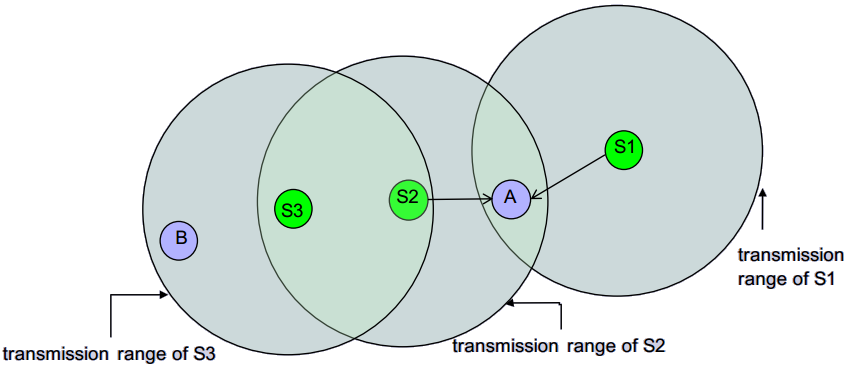
\includegraphics[scale=0.7]{img/manet}	
\caption{Example topology of a MANET}
\end{figure}

\subsection{Data Mining and Monitoring}
The core functionality of MANETs is to provide a network of mobile nodes which can communicate with one another and pass information by routing through intermediate nodes where necessary. In a sensor network, each node is tasked with collecting specialised data through the use of sensory peripherals, and this data must be passed effectively to its destination. Given the dynamic nature of MANETS, considerations must be made for the constant changing topology in order to ensure that the networks's integrity and availability is not compromised and that nodes can effectively communicate with one another at any time \cite{ramramathanjasonredi2012}. This includes problems such as losing connection or going out of range, which will cause the loss of packets when communications links are inevitably cut and messages lost. 

Connections between nodes and algorithms for data mining must be carefully established and monitored in order to ensure secure and efficient routing. For example, the data collected by each individual sensor node which is monitoring an environmental feature will typically register similar values due to spatial correlation, so there is a danger for unnecessary overheads as a result of unneeded data. By measuring spatial correlation between data sampled by different sensors, specialised algorithms can be developed to implement more efficient data mining, as well as optimising routing strategies \cite{mayajie2011}. In order to aggregate data more effectively, a  stationary base station node may be included, which acts as the data sink, and may be capable of passing user input to nodes, which would allow for some stability and interaction with the network by the user. 
POSSIBLE OBLIGATORY IMAGE OF BASE STATION NETWORK/BROKEN LINKS

\subsection{Sensor Networks}
A sensor network is different to a simple MANET in that each node has autonomous sensors to monitor physical or environmental conditions such as temperature, sound or pressure. This data can also be routed through other nodes, and it may be possible to control sensor activity if networks are bidirectional \cite{kazem2007}. While sensor networks themselves can range from wired to wireless, or have predefined topologies such as the simple star network or a multi-hop wireless mesh network, a drone sensor network would be classified as a mobile wireless sensor network (MWSN) for obvious reasons. 
The biggest challenges to MWSNs, in general terms, are hardware and environment. Power consumption of the sensing device should be minimised and sensor nodes should be energy-efficient, since their limited energy resource determines their lifetime. As with any mobile network, the varying topology due to the mobility of nodes results in further usage of the already limited resources in terms of battery power. If it is possible, nodes could consider powering off unused parts to save power, such as immediately after takeoff, where sensors may not be required en route to the target area. However, this is also dependent on the environment, which may require additional precautions in the event that it is hazardous or requires heavy monitoring. The most effective method for energy efficiency is the use of optimal routing protocols, which will be discussed in later sections \cite{shiny2012}.

\section{Simulations}
\label{simSoft}
Network simulators are software that predict the behaviour of a computer network, making them a popular method for experimentation with a possible model for MANETs due to their ability to cheaply and flexibly model a solution. These simulation tools make it possible to model fault tolerance, scalability, make monitoring easy, and provide reproducibility \cite{stuartkurkowski2005}. It should be noted that there are significant variations in the way that individual simulators operate, which cannot be expressed in terms of accuracy. At best, they can be said to be dependable and realistic with reasonable proficiency at modelling unpredictable error in a real environment. Simulation events can be split into continuous and discrete simulation, where continuous simulation makes use of analytic models, and so can hardly be applied in practice. Conversely, discrete simulation allows for parallelism, scalability, and speed up, as well as developing trace files containing a description of each event that occurred \cite{luchogie2006}. These trace files can then be used to generate a visualisation of the simulation, so they would be preferred for our project (or they will influence how we build our simulation and visualise it). This section gives an overview of the potential solutions available for simulations, and the alternatives to using a simulator.

\subsection{ns-2}
ns-2 (network simulator) is a discrete-event network simulator, for research and educational use. Its software infrastructure encourages the development of simulation models which are sufficiently realistic to allow it to be used as a real-time network emulator, and is the basis for many existing real-world implementations \cite{tommasopecorella2016}. In particular, it provides a set of randomised mobility models, including random waypoint, such that the advanced node mobility constitutes a progression towards realistic simulation. ns-2 programs are scripted in OTcl, with some components written in C++ . Despite its popularity, ns-2 suffers for its lack of modularity and inherent complexity, but does provide excellent documentation. It is the predecessor of ns-3, although it has a greater diversity of models given there more years of contributions. ns-2 also allows for visualisation of the simulation through its GUI out.nam with the use of trace files, as shown in figure \ref{outnam} \cite{luchogie2006}.

\begin{figure}
\centering	
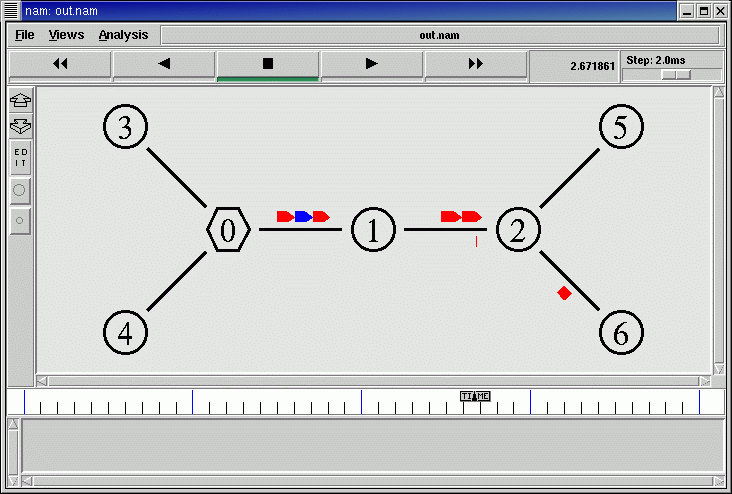
\includegraphics[scale=0.4]{img/outnam}	
\caption{ Visualisation for ns-2 trace files in out.nam}
\label{outnam}
\end{figure}

\subsection{ns-3}
ns-3 is a new software development which followed  ns-2, focusing its efforts on improving the core architecture, software integration, models, and educational components of ns-2 \cite{ns2006}. ns-3 differs from ns-2 in that it is purely written in C++, with optional Python bindings. New scripts can therefore be written in C++ or in Python. This version is recommended over ns-2 by the creators of ns due to features which are not available in the previous version, such as an implementation code execution environment, which allows users to run real implementation code in the simulator. Additionally, it has more detailed models, as well as being actively maintained and developed. ns-3 is not backwards compatible with ns-2; it is an entirely new simulator, with several models which were written in C++ which are already been ported to ns-3 \cite{tommasopecorella2016}. The visualisation platform for ns-3 is the animator NetAnim, shown in figure \ref{netanim} based on the Qt toolkit.

\begin{figure}
\centering	
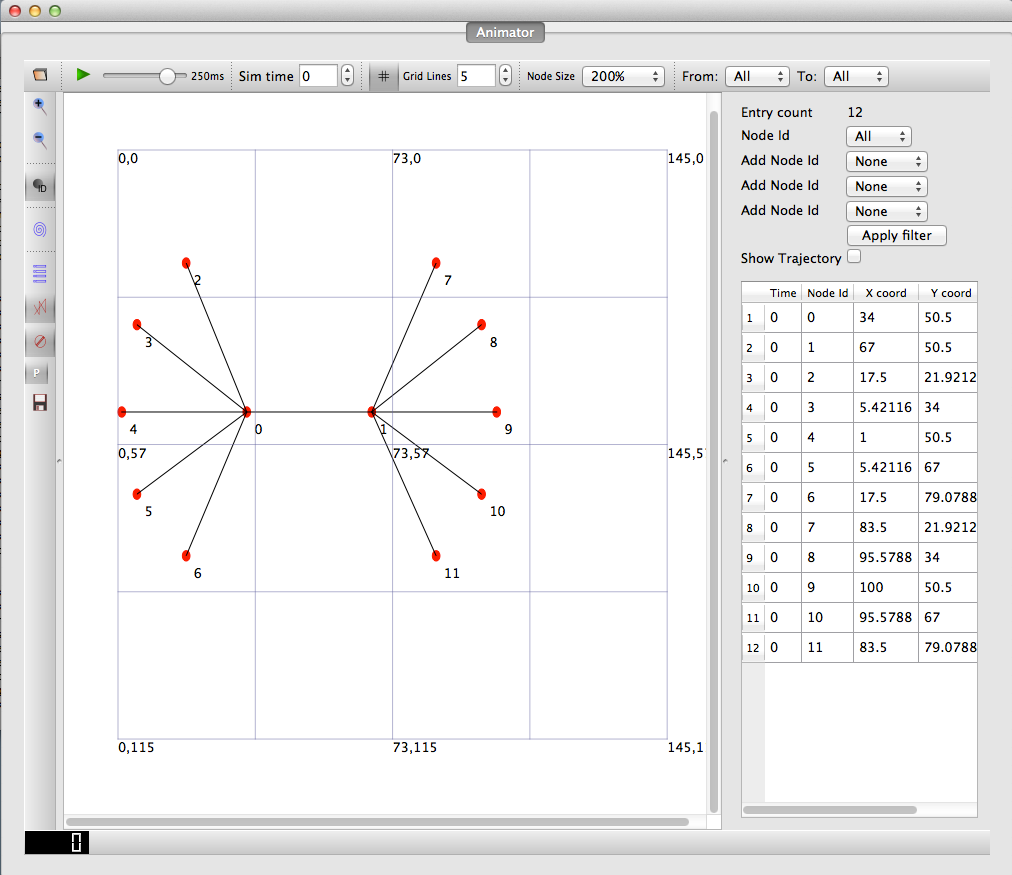
\includegraphics[scale=0.3]{img/netanim}	
\caption{An example of NetAnim simulation animation}
\label{netanim}
\end{figure}

\subsection{GloMoSim}
Short for Global Mobile Information System Simulator, GloMoSim is a network protocol simulation software for parallel simulation of wireless and wired network systems using the parallel programming language PARSEC \cite{zengxiang1998}. It uses a message-based approach to discrete-event simulation, where network layers are represented as objects called entities, which handle events represented by timestamped messages. The library has been designed to be extensible and composable, and its modular implementation enables consistent comparison of protocols at a given layer. While research into parallel simulation is relatively limited, and areas such as signal interference and attenuation are inherently more complicated, there are clear implications for a significant increase in performance in terms of spreading out the simulation overheads, which may outweigh the inherent complexity. The PARSEC Visual Environment (PAVE) shown in figure \ref{pave} has also been developed to support the visual design of GlomoSim event simulations \cite{luchogie2006}.

\begin{figure}
\centering	
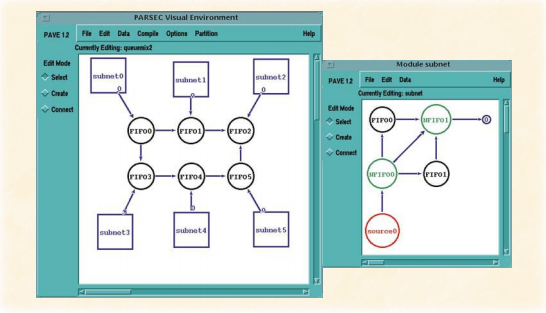
\includegraphics[scale=0.8]{img/pave}	
\caption{Example output from the PARSEC Visual Environment}
\label{pave}
\end{figure}

\subsection{OMNet++}
OMNet++ is an extensible, modular, component-based C++ simulation library and framework, primarily for building network simulators \cite{omnet2016}. This includes wired and wireless communication networks for sensor networks, ad hoc networks, Internet protocols, and so on. OMNet++ is not a network simulator in and of itself, but provides a wide range of tools and extensions, including an Eclipse-based IDE (Integrated Development Environment). It provides a component architecture for models; components are programmed in C++ and then assembled into larger components and models using a high-level language (NED) which also has GUI support, as shown in figure \ref{omnet}. OMNet++ was designed for the general use case, as opposed to being a specialised simulator, and its modular architecture allows for the simulation kernel (and models) to be easily integrated into wider systems \cite{varga2008}. 

\begin{figure}
\centering	
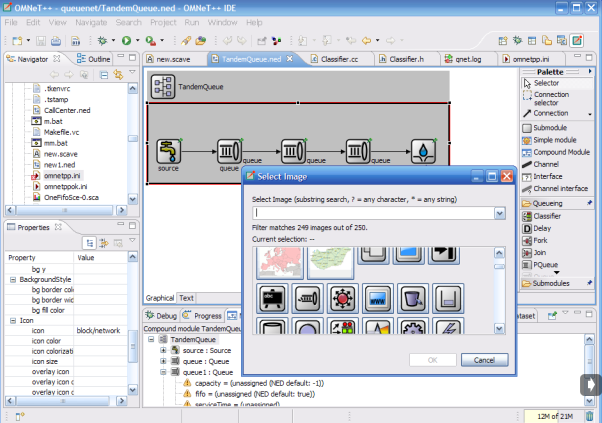
\includegraphics[scale=0.7]{img/omnet}	
\caption{Example of the OMNet++ NED editor IDE}
\label{omnet}
\end{figure}

\subsection{Testbeds}
As an alternative to simulations, testbeds are in-lab networks built and used by researchers, which involves creating and connecting physical devices for testing the application of real networks. As a result, the cost of hardware coupled with the difficulty of managing applications in terms of deployment and monitoring creates limitations on the complexity and scalability of the network. While it can be said that the physical testing environment is much more effective and realistic than a simulation, the lack of larger testbeds of over 50 nodes prevents this from becoming a major component for validating new concepts and applications for MANETs \cite{luchogie2006}.

\section{Drones}

\subsection{UAV Components}
As has been discussed in previous chapters, drones have a variety of sizes, utilities, costs, and applications, from commercial to military purposes. However, they will all have to make use of sensors, actuators, software, and a power supply in battery form. The body includes a fuselage and wings for planes, tail rotor for helicopters, and a frame and arms for multirotors \cite{mitchjohnson2015}. The combination of different layers of computer software with different time requirements, also referred to as the autopilot or flight stack, may require specialised externally supported hardware such as Raspberry Pis or Beagleboards. This is because on-board classical operating systems may be too intensive for some embedded systems, presenting problems if the aircraft is dependent on fast response times \cite{paparazzi2016}. 
Depending on its usage, a drone will also range from being fully remotely piloted to complete autonomy such that the drone will function without any user input. Is important to note that the degree of autonomy i.e. the extent to which the aircraft is independent from operator assistance, is different to the level of autonomy in terms of the scope of tasks it can perform and their sophistication \cite{williammarra2012}.

\subsection{Drone Autonomy}
Autonomy is split into different layers of control, from basic manoeuvrability and flight controls to system management, navigation and mission planning. It is assumed that the user will be able to provide task level instructions which the drone is capable of processing. The figure below shows an example of the basic autonomy controls for a UAV.

\begin{figure}
\centering	
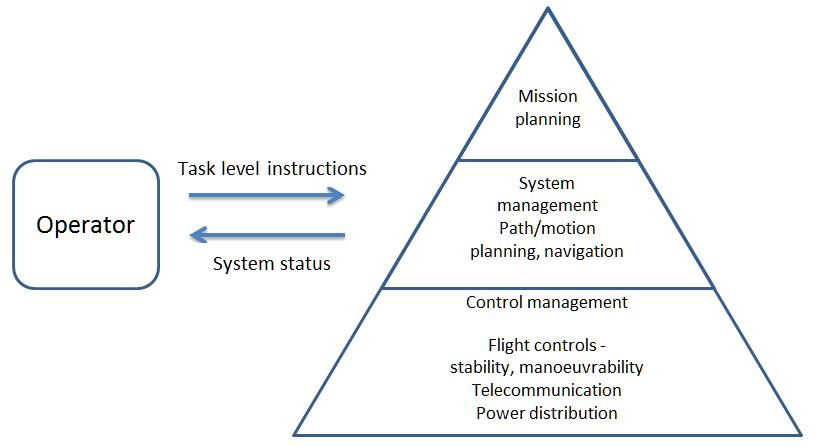
\includegraphics[scale=0.4]{img/autopyra}	
\caption{Hierarchy of drone autonomy and user control}
\end{figure}

An autonomous drone would be expected to have various features for flight control and communications, such as:
\begin{itemize}
\item \textbf{Autonomous takeoff and landing}
\item \textbf{The ability to return to its starting location}
\item \textbf{A failsafe to autonomously land the drone in the event of loss of signal}
\item \textbf{The ability to stabilise and maintain altitude in unstable conditions i.e. hover and self-level in wind}
\item \textbf{Possible GPS waypoint navigation}
\end{itemize}
A drone will already contain a microcontroller often with pre-programmed instructions for navigation, including tricks such as rolls and loops; however, an external small computer would be required to implement mid-level algorithms such as those involved in physical routing and communications. For example, determining an optimal path whilst avoiding obstacles, or passing messages in a network to other nodes. The attachment of an external computer such as a Raspberry Pi would allow for the drone to be programmed directly, which is the most common solution achieving autonomy (discussed later).
Reactive autonomy, such as real-time collision avoidance, relies on situational awareness, which is typically provided by range sensors. However, a network of drones with GPS capabilities would be able to utilise its own spatial awareness, knowledge of other node positions, and protocols designed to avoid collision. 

\subsection{Classifications}
UAVs have been classified by such areas as weight, functionality, range and usage. Given that this project focuses on the use of consumer-level drones, we will focus on the classification of drones by usage \cite{yashgarg2015}. The fundamental types of drones are as follows:

\begin{itemize}
\item\textbf{ Commercial off-the-shelf (COTS).} This refers to drones which are ready to fly immediately with no prior or specialised knowledge required
\item\textbf{ Bind-and-Fly (BNF) and Almost-Ready-to-Fly (ARF).}  BNF and ARF drones typically contain most or only some of the parts required for the drone, but may be missing components such as the controller or battery, and require some knowledge to assemble and configure
\item \textbf{Midsize Military and Commercial Drones.} These drones are more expensive, with greater utilities and/or bespoke functionality
\item \textbf{Large Military-Specific Drones.} Military drones may be used for combat, logistics, research and development, reconnaissance or as target and decoy drones
\item \textbf{Stealth Combat Drones.} Military drones which are used for stealth operations, including direct combat and reconnaissance

\end{itemize}
For a drone sensor network, it is important to be aware of power consumption, the weight, and the range of the drone in order to maximise its efficiency and understand the limitations of a single drone in the network. COTS drones (or quadcopters) will typically carry a payload (such as a camera), and additional peripherals such as the external computer required for implementing autonomy and sensing equipment will add to the weight of the drone, so considerations must be made for load capacity. Additionally, range will be directly influenced by the choice of medium, such as Wi-Fi or radio. All of these additions to the drone will affect the ‘Degrees of Freedom’, which is the number of axis and sensors combined for balancing a plane, helicopter or robot, which typically is equated with the complexity (and therefore, price) of a UAV \cite{arduinodof2012}.

\section{Existing Solutions}
This chapter has researched the structure and characteristics of sensor networks, including implementation and testing through simulators, as well as examining different varieties of drones and their components, identifying how this can be related to sensor networks. This section will highlight some of the advances and complications which arise within sensor networks, autonomous drones, and explicit combinations of both, by examining existing implementations and research into the field.

\subsection{Autonomous Drone Implementation}
UAVs and autonomous aircraft have become increasingly popular as an area of research and development, and a number of open source autopilot projects exists which can facilitate autonomy, allowing hobbyists and businesses to use them on small, remotely piloted aircraft inexpensively. Among these are GPS-based projects such as Paparazzi and ArduPilot, which will be analysed to see how they can be applied to drones, and how they differ in terms of their choice of operating system and implementation. Other methods of achieving drone autonomy will also be discussed in this section.

\subsubsection{Paparazzi}
Remes et al. \cite{bartremes13} conducted studies on the use of a GPS-based open source autopilot system known as Paparazzi in order to create a swarm of autonomous Parrot AR drones. The Parrot firmware can be enhanced with Paparazzi firmware, or a standalone version of the Paparazzi firmware can be used. The autopilot will lock onto sufficient GPS satellites, establish a signal and enact a user constructed flight plan.
Paparazzi includes a base station GUI known as the Ground Control Station (GCS) for the purpose of preparation, simulation, monitoring and analysis, and each drone can be located on the map provided.  The overlay includes information about the drones such as height, waypoints for the flight plan and controls. The addition of more drones is arbitrary; installing the firmware on each drone will allow it to be located on the GCS and interacted with. 

\begin{figure}
\centering	
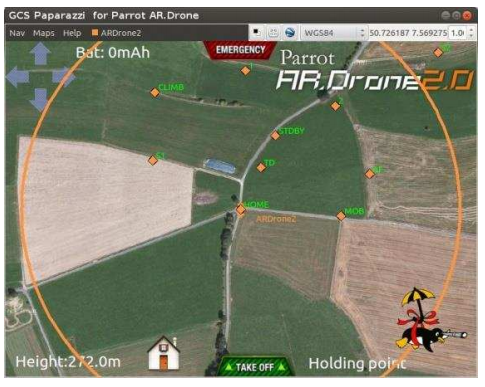
\includegraphics[scale=0.4]{img/papgcs}	
\caption{The Ground Control Station of Paparazzi for the Parrot AR drone 2}
\end{figure}

Both inner and outer loop control is performed by Paparazzi, which means that the flight plan controls the thrust and attitude for achieving the right speed and position, and the safety pilot has control over the vehicle via the RC link, which refers to the joystick connected to the GCS. The control loops are open source, however, and can be changed by the user.

\begin{figure}
\centering	
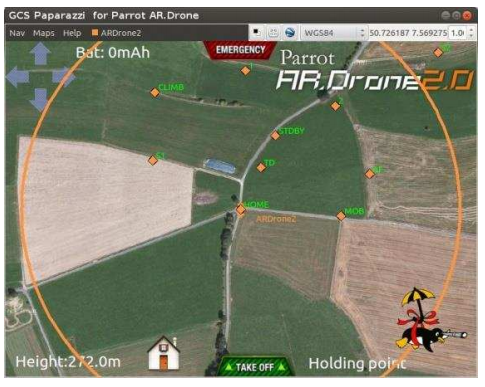
\includegraphics[scale=0.4]{img/papgcs}	
\caption{Global view of the control loops used by the Paparazzi airborne code for navigation, guidance and control}
\end{figure}

\subsubsection{Ardupilot}
He Bin et. al \cite{ hebin2009} discuss the design, modelling, implementation and testing of an autonomous UAV with the use of Ardupilot, which is another open source UAV autopilot platform. Ardupilot is a portmanteau of Arduino and pilot, the former being open source electronics prototyping platform upon which Ardupilot is based. It is similar to the Paparazzi project in terms of its free software approach and GPS-based implementation. 

\begin{figure}
\centering	
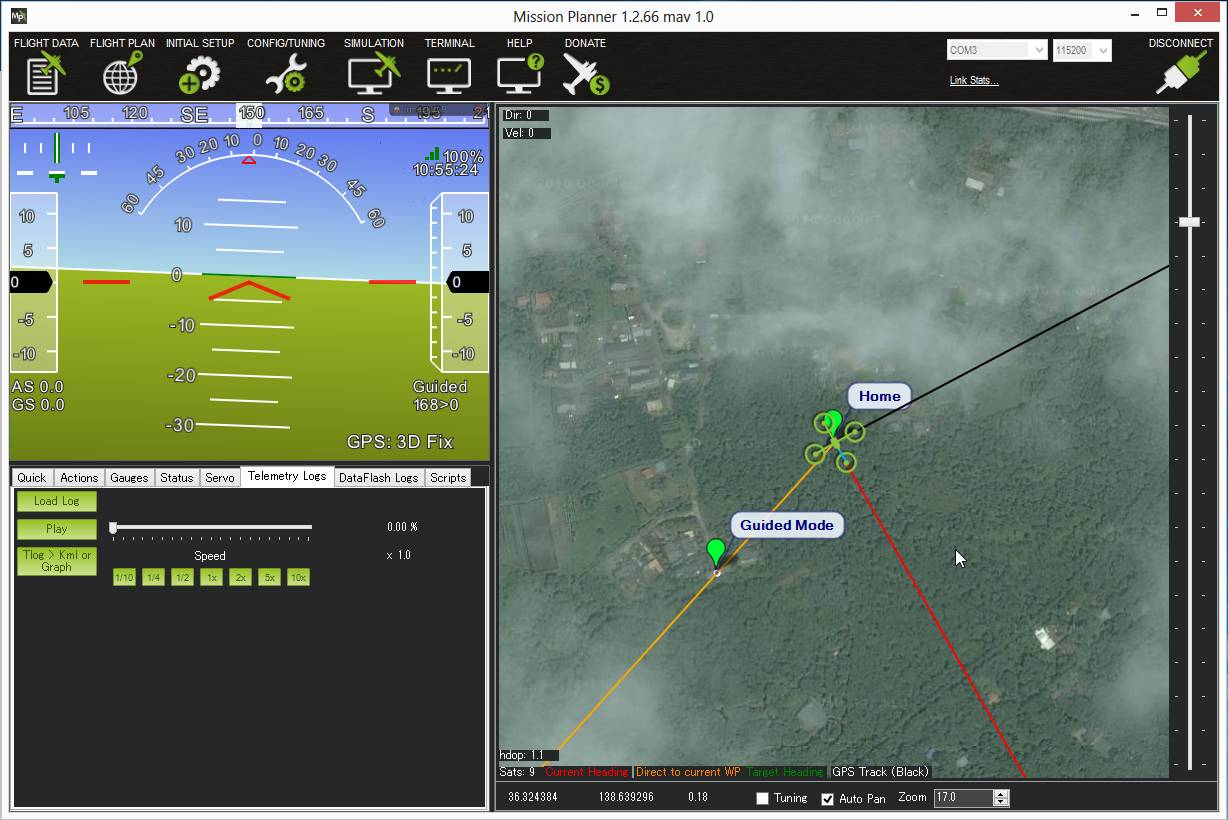
\includegraphics[scale=0.2]{img/ardgui}	
\caption{Example output of  the Ardupilot Mission Planner software}
\end{figure}

The Ardupilot is a custom PCB with an embedded processor combined with a built-in hardware failsafe to switch between RC control and autopilot control, such that the user can decide the amount of direct control over the UAV themselves. The autopilot controls navigation (by following GPS waypoints) and altitude by controlling the rudder and throttle.
The Ardupilot software is an open source Arduino environment which can be easily run and edited on Windows, Mac OS X and Linux, in contrast to Paparazzi, which runs exclusively on Ubuntu, and requires more specialist knowledge (including a reasonable grasp of the command line). However, it requires for waypoints to be set manually and before takeoff, which limits the level of autonomy which can be achieved. Ardupilot is widely regarded as the ‘breakout’ model for autopilots, due to its ease-of-use and price (which is much cheaper than Paparazzi), with somewhat reduced functionality and lower specs.

\subsubsection{Map Stitching}
In order to solve the problem of autonomous drone control, Visser et al. introduce a method of navigation using image stitching to build a visual map of an indoor environment \cite{arnoudvisser2011}. Using the frames from the Parrot AR Drone’s (which we are using for the project) downward-facing camera, sets of matches between two camera frames are used to estimate a tomographic model for the apparent image motion. Thus, a model can be composed with the estimated motion of the rest of the images in order to build a mosaic. Additionally, it makes use of sonar sensor input to detect obstacles which are then added to the camera image during the image stitching process. An example result of the map stitching is shown in figure \ref{fig:mapstitch}.

\begin{figure}
\centering	
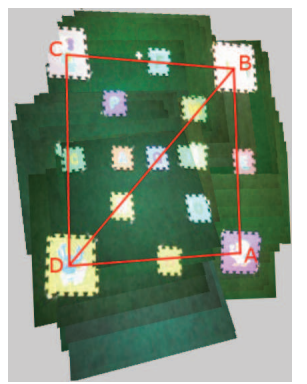
\includegraphics[scale=0.2]{img/mapstitch}	
\caption{Map created by the map stitching method using camera images taken by the AR drone }
\label{fig:mapstitch}
\end{figure}

Calculations for frames are further influenced by a number of additional sensors such as inertial sensor data, which can be used to estimate current position, calculate an estimate for the resulting position, and use this as input for the map stitching algorithm. 
**MATHS AND ALGORITHMS HERE?**
Results showed that the visual map created by a simulated AR drone contained fewer errors than a map from the real drone, which could be attributed to the effect of automatic white balancing of the real camera. However, the map stitching method is able to map small areas visually with sufficient quality for human navigation.

\subsubsection{Drone Localisation}
Dijkshoorn et al. \cite{dijkshoorn2011} introduce a similar method for autonomous navigation which uses sensor and motion models to localise an autonomous Parrot AR drone. This method involves creating a visual map using texture and feature mapping derived from the position and attitude of the drone in the world, whereupon the map can be used for absolute position estimates and subsequent navigation. By creating a visual map, it is possible to sufficiently conduct human and artificial navigation through an indoor space. Simulation of the AR drone is also performed to aid in the estimation and testing of localisation methods and mapping.

\begin{figure}
\centering	
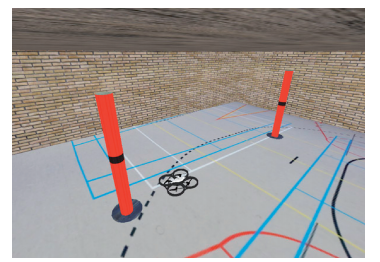
\includegraphics[scale=0.7]{img/dronemod}	
\caption{3D model of a gym with realistic ground and wall textures for AR drone simulation}
\end{figure}

Firstly, to initialise the visual localisation and mapping algorithm, the internal sensors of the drone are used to give information about the position and movement of the drone. The inertial sensor measures body acceleration and angular velocities, which can be converted to an estimated attitude. Sonar sensor is used to measure the altitude of the drone, and an estimation of body velocity is calculated using inertia measurements and optical flow from the relative motion between camera frames. This information is used to build a visual map of the environment.
**MORE MATHS HERE MAYBE**
Results showed that the mapping method is able to map areas visually with sufficient quality for both human and artificial navigation purposes. The simulation contained fewer errors than the real Parrot AR drone, which were attributed to measurement noise, however, the localisation and visualisation methods were demonstrated to make autonomous navigation possible

\subsection{UAV Sensor Networks}

\subsubsection{Collaborative Drone Tasking}
Recognising the difficulty in coordinating multiple drones to perform a task collaboratively in a sensor network, Mottola et al. \cite{mottola2014} introduce and provide an analysis of the concept of team-level programming, which can express collaborative sensing tasks without the complexity of such areas as concurrent programming or parallel execution. They create the VOLTRON programming system to explore this concept and enable coordination of multiple drones with a specific focus on active sensing applications, and dynamic re-tasking.
This method of team-level programming was developed in contrast to drone-level programming and swarm programming, which focus on addressing and tasking each individual drones with navigation, communication, and sensing, or executing a single set of basic rules and operating only on their own local state, which is difficult to scale up to multiple drones. Team level programming allows for sophisticated collaborative sensing tasks without resorting to individual addressing, enables simpler code execution, and produces marginal overhead in terms of CPU, memory and network utilisation.
Mottola et al. concluded that the implementation of a team-level programming model in VOLTRON provided a significant improvement in execution time for a given task when using multiple drones. Application level performance of real-time drone applications were assumed to depend greatly on hardware design choices and execution times could be variable depending on the environment. Nonetheless, the use of a testbed, as well as real deployment, produced results that VOLTRON does introduce overhead, but that memory consumption and CPU utilisation are independent of the number of drones, and this system would likely scale effectively beyond 100 drones before reaching resource limits. 
**POSSIBLE COMPARISON BETWEEN DIFFERENT IDEAS?/HOW WE FEEL ABOUT THIS**

\subsubsection{Emergency Services}
One of the most common applications of UAVs aside from commercial or military is in the field of disaster prevention, management and relief. FUEGO, the Fire Urgency Estimator in Geosynchronous Orbit, is a system created by researchers at UC Berkeley which locates and identifies fires using drones, planes and satellites with special infrared cameras \cite{shelbycarpenter2015}. The network of drones will navigate through fire-prone areas of the country, taking photos at a wavelength of light that fire emits, but which is invisible to the human eye. A geospatial information system (GIS) processes the images in real time to estimate the risk that a hotspot could grow into a serious fire, where the difference in each sample can highlight the eruption of a forest fire. With this system, it is possible to identify forest fires within 3 minutes of their eruption \cite{fuego2015}.
Research into the application of networked UAVs for disaster management is also being conducted to test the ability of small-scale, battery-powered, and wirelessly connected UAVs carrying cameras for disaster management, such as a wood fire or a large traffic accident, and deliver high-quality sensor data such as image or video. Quaritsch et al.\cite{quaritsch2010} discuss the potential of the tight integration of sensing and controlling UAVs, which allows for a whole new set of applications and research challenges. Following disasters such as Hurricane Katrina, UAVs were equipped with a digital camera capable of both still and video imagery for post-disaster data collection and damage inspection of multi-storey commercial buildings \cite{stuartadams2011}. The most prominent challenges to UAV sensor networks are described as optimisation for area coverage, as well as concerns over limited resources, especially energy. Limited site access and landing and takeoff environments also required that there were greater flight distances to reach areas of interest, which further emphasises the importance of energy efficiency. 

\section{Routing}
Two of the biggest challenges for UAV Sensor networks which have been introduced so far are the issues of limited resources and the environment. In order to minimise overheads, reduce computation time, optimise pathing and battery usage, and introduce energy-efficient communication, it is essential to consider different methods of routing in sensor networks. The length of operation time and success of the network relies on firmly established protocols which are optimised for the application. In this section, we examine some of the existing algorithms for routing, giving a brief discussion of the advantages and disadvantages of each method and how they deal with specific challenges such as robustness and energy efficiency. 

\subsection{Ad Hoc On-Demand Distance Vector}
Ad Hoc On-Demand Distance Vector (AODV) routing is a non-position based protocol which enables dynamic, self-starting, multi-hop routing between participating mobile nodes. It operates by sending Route Request (RREQ), Route Reply (RREP) and Route Error (RERR) messages between nodes, which are used to establish endpoints of a communication connection (as shown in figure \ref{aodv}).  In AODV, the source node and the intermediate nodes store the next top information corresponding to each flow for data packet transmission \cite{perkins2003}.

AODV is a reactive (on-demand) routing protocol in that it does not do anything if an active route already exists between communicating nodes, so connection setup delay is less, and destination sequence numbers are used to find the latest route to the destination. The AODV protocol also keeps the overhead of messages small, and has a great advantage in overhead over simple protocols which need to keep the entire route from source to destination in their messages. This protocol is also loop-free and avoids the counting to infinity problem through the use of sequence numbers. Despite this, such protocols have a high latency time in finding a route (because routing is done in reaction to a message being sent), and excessive flooding can lead to network clogging. 

More information about AODV can be found in section \ref{AODVdesc}.

\begin{figure}
	\centering	
	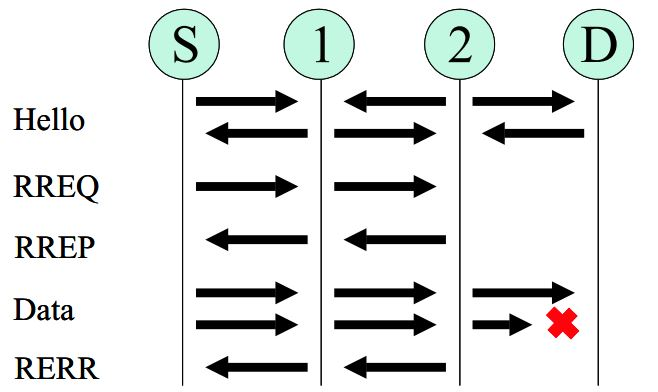
\includegraphics[scale=0.7]{img/aodv}
	\caption{Packet delivery rate for a 50 node model (30 traffic sources)\cite{chakeres2004aodv}}
	\label{aodv}
\end{figure}

\subsection{Dynamic Source Routing}
Like AODV, Dynamic Source Routing (DSR) is an on-demand routing protocol for mobile ad hoc networks. DSR divides the routing problem into two parts: route discovery and route maintenance. Route discovery finds routes between nodes by flooding the network with discovery packets until the destination node is reached. A route reply message is propogated back and cached. Unlike AODV, routes are retained indefinitely (unless they are broken), meaning that when nodes are static the overhead from using DSR is zero\cite{Johnson01dsr:the}\cite{johnson2007dynamic}.

Route maintenance is performed whenever a data message is being sent through the network. Each node is responsible for ensuring that messages it forwards are received (this is often done through link-level protocols or passively on retransmission). In the event of a link being severed and a message being lost, the node which attempted to send over the broken link returns a route error message to the originator of the message. Routes using this link are removed from the cache.

One of the advantages of DSR is that new routes and network updates are retained by every node which witnesses them (each node a route error message passes through will remove the broken link from their routing cache). Additionally, DSR nodes will attempt to shorten routes, salvage packets sent over broken links, and reason about link uni/bi-directionality. This focus on preventing the duplication of messages means that DSR is fast with very low overhead.

\subsection{Greedy Perimeter Stateless Routing}
Greedy Perimeter Stateless Routing (GPSR) take a different approach to routing than AODV and DSR in that it is stateless. Instead of using caching to reduce the amount of overhead, each node memorises the geographical locations of its neighbours and uses this to greedily forward messages. The optimal (one hop) choice for routing is the neighbour which is closest to the destination node\cite{karp2000gpsr} (see figure \ref{gpsr1}).

\begin{figure}
	\centering	
	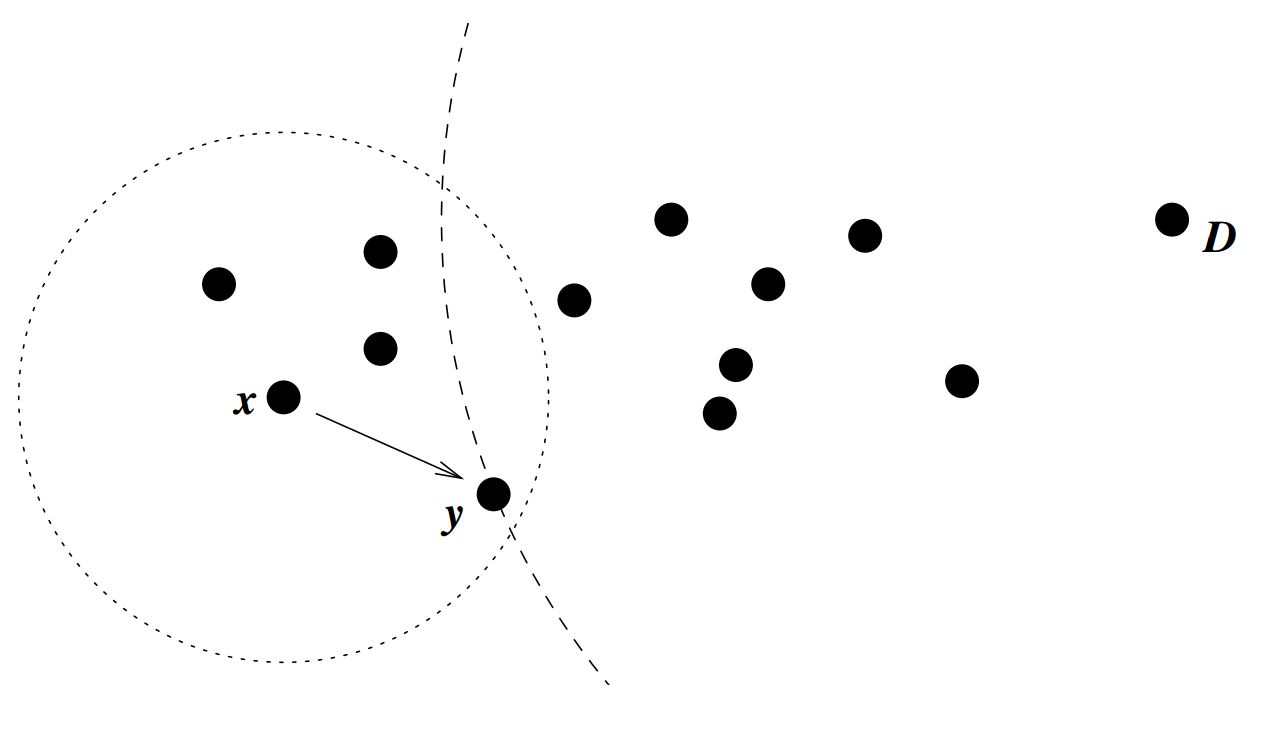
\includegraphics[scale=0.7]{img/gpsr2}
	\caption{An example of greedy forwarding in GPSR\cite{karp2000gpsr}}
	\label{gpsr1}
\end{figure}

The disadvantage of retaining as little information as possible is that there is an associated messaging overhead. GPSR nodes will routinely beacon information about their location, though can be mitigated through the practice of attaching beaconing information to all packets sent. This is exactly what AODV and DSR explicitly try and avoid through the use of caching. There are also scenarios where the optimal node to forward to is not the one chosen by the greedy algorithm. In this case, the right hand rule is used to route packets to their destination.

Benchmark simulations of GPSR and DSR reveal that the overhead incurred by beaconing is normally less than that of more stateful solutions, as shown in figure \ref{gpsr2}. It is worth noting that 

\begin{figure}
	\centering	
	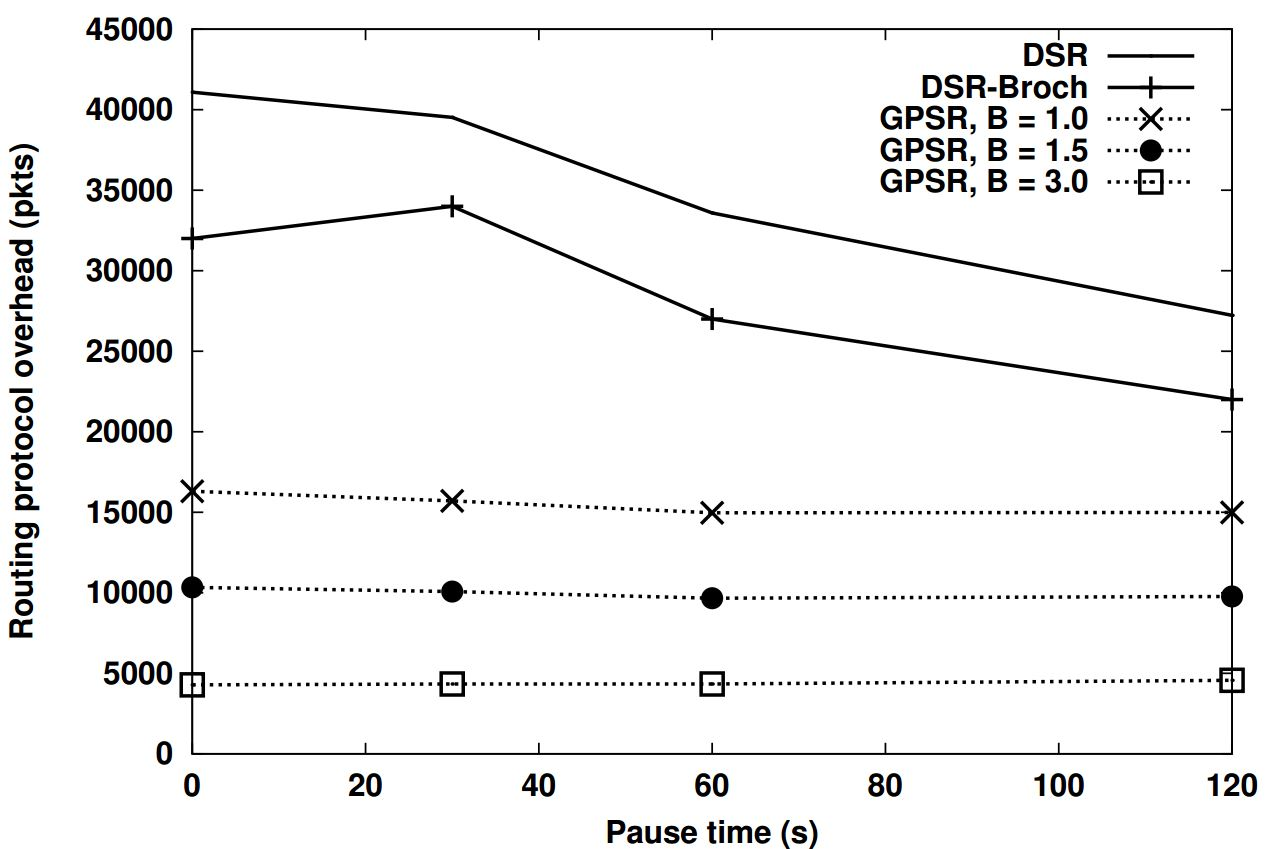
\includegraphics[scale=0.7]{img/gpsr}
	\caption{A comparison between DSR and GPSR with different beaconing intervals $b$\cite{karp2000gpsr}}
	\label{gpsr2}
\end{figure}	
	
\subsection{Comparison}
Figures \ref{dsraodv1}, \ref{dsraodv2}, and \ref{dsraodv3} show a comparison between AODV and DSR in similar conditions. It can be seen that DSR tends to perform better in terms of overhead when considering short pause times (typical of a drone network), but that AODV results in a higher percentage of packets being delivered. Given the need for high priority messages to be delivered as quickly as possible in a quadcopter network (to prevent a collision, for example), it was decided that AODV would be a more appropriate algorithm to implement as a reference communication model in octoDrone than DSR. GPSR is very efficient but suffers from the problem that geographic routing tends to break down when nodes are moving at high speeds most (if not all) of the time. As information on neighbours becomes less certain it is harder to make efficient routing decisions without drastically decreasing the broadcast interval. After some consideration it was decided that AODV would be more broadly applicable, with GPSR being a worthwhile future addition.

\begin{figure}
\centering	
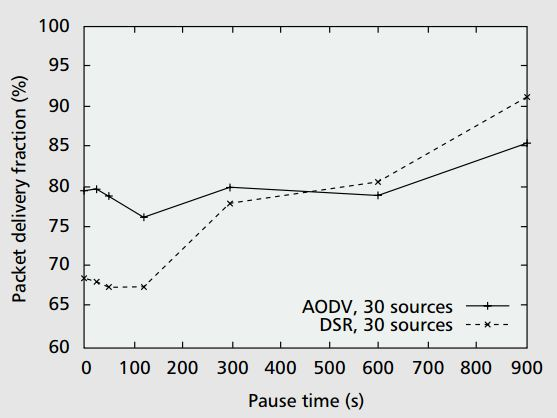
\includegraphics[scale=0.7]{img/comp1}
\caption{Packet delivery rate for a 50 node model (30 traffic sources)\cite{perkins2001performance}}
\label{dsraodv1}
\end{figure}
	
\begin{figure}
\centering	
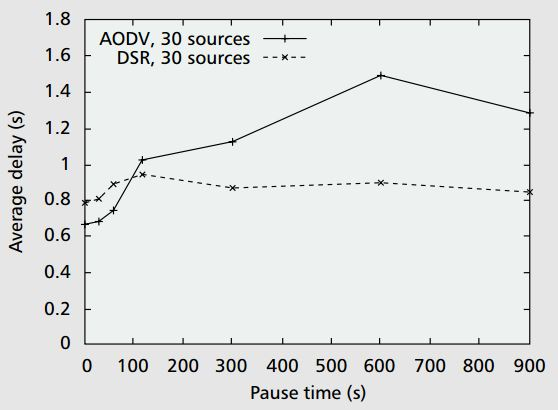
\includegraphics[scale=0.7]{img/comp2}
\caption{Average data packet delay for a 50 node model (30 traffic sources)\cite{perkins2001performance}}
\label{dsraodv2}
\end{figure}
		
\begin{figure}
\centering	
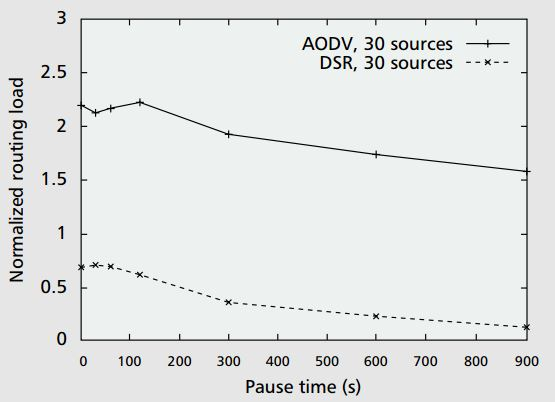
\includegraphics[scale=0.7]{img/comp3}
\caption{Normalised routing load for a 50 node model (30 traffic sources)\cite{perkins2001performance}}
\label{dsraodv3}
\end{figure}
	
\section{Social and Ethical Issues}
The subject of drones has been the focus of much controversy with regards to issues of privacy, invasion of airspace and other unsanctioned uses of UAVs with the ability to, for example, use a camera to take pictures or video. Therefore, a platform for an entire network of drones with a variety of sensors which is open source presents a multitude of possible problems. Furthermore, with the potential to be used as a foundation for military efforts, which form the basis of many current topics of research into drones and sensor networks, there are many implications for potential misuse of the project. As a result, it is necessary to research and discuss the possible methods of unlawful utilisation of drones and drone networks, in order to ensure that the project group is aware of these issues.

\subsection{Privacy}

\subsubsection{Spying}
Freedom of information has been a topic of discussion with regards to the ability to use drones with cameras attached which could be classified as an invasion of privacy. In the UK and the US \cite{rebeccarosen2013}, there has been a huge spike in drone-related incidents. Examples include drones flying and photographing over private property, and hovering in front of the windows of a property with the camera facing inside the window \cite{maryannrusson2015}. It is difficult to argue what constitutes an invasion of privacy, particularly when the law regarding UAVs has yet to be refined in order to reflect the advancement of technology. 
The law is, however, very clear with regards to the use of firearms against UAVs, whether or not the UAV in question was trespassing or invading on private property. In November 2014, a man was fined \$850 in damages for shooting down a neighbour’s drone while it was flying over the neighbour's property, and then refusing to pay any compensation for destroying the drone \cite{colinneagle2015}. The Federal Aviation Administration’s (FAA) definition of a drone as aircraft also means that, technically, shooting a drone could result in a maximum penalty of a 20 year prison sentence. Pursuing legal action in cases such as this is difficult, as it is not illegal to fly a drone in public.

\subsubsection{Data Collection}
A more prevalent issue arises where any drone carrying a payload such as a camera has the potential for recording data unlawfully. In one instance, a drone which was found to be hovering over an ATM that seemed to be recording people entering their pin numbers into a cash machine. It can be argued that the drone was not breaking the law by simply recording a public space\cite{maryannrusson2015}. However, it is difficult to prove that the usage of the drone was for the express purpose of obtaining peoples’ pin number, or if this is unlawful to begin with, in the same way that there is no law which expressly forbids someone from looking over the shoulder of an ATM user.
A full-length documentary called Speciesism: The Movie based its foundational discoveries and source of information by using drones to spy on factory farms and record evidence of environmental damage, and went on to feature major global press coverage. In this particular instance, the law with regards to prosecution was unclea, despite the activity being labelled as ‘spying’. This could suggest that such uses of drones, even on potentially private property, may not be possible to prosecute, although this may be unique to incidences of whistleblowing.
** PICTURE OF SPYING IMAGE?**

\subsubsection{Unsanctioned Airspace}
There are several instances where the definition of misuse of drones has been well established and offenders have been prosecuted. In the very first case of prosecution against unsanctioned drone usage, a security guard was sentenced after repeatedly flying drones over and around Premier league football stadiums, Buckingham Palace and Parliament buildings, where he was fined and banned from flying UAVs \cite{maryannrusson2015}.  In the US, FAA regulations state that drones must not be flown near airports and other areas with manned aircraft, as well as placing a ban on altitudes over 400ft. The Civil Aviation Authority (CAA) in the UK states that for a Small Unmanned Surveillance Aircraft (SUAS) of less than 20 kg, the operation must not endanger anyone or anything, and the aircraft must be within visual line of sight \cite{civilaviationauthority2015}.
For the specific case outlined above, the aircraft being used for surveillance purposes was in violation of the rules of direct line of sight of the aircraft as well as being subjected to tighter restrictions with regard to the minimum distances that you can fly near people or properties that are not authorised. In most instances of prosecution, the owner of the drone would be required to have permission from the CAA to fly their drone in an area that would usually be forbidden access.

\subsection{Military Use}
As discussed in previous sections, engaging in military operations is one of the most prevalent uses for drones, as well as being a popular area for research and development of UAVs. Fortunately, the specifications of consumer-level drones are not of a high enough calibre to warrant usage in the military, which requires state-of-the-art hardware, including weaponry. However, there is an initiative to create small, hand-sized mini drones for soldiers in the US Army, for the purpose of small scale intelligence gathering and reconnaissance, in place of conventional air support \cite{jonfingas2016}. Projects such as this have implications for the usage of drones of all shapes and sizes in military operations, which would suggest that implementations of drone autonomy by hobbyists and businesses may form a basis for research and development in the army.
The use of drones for spying is not only limited to consumers, militaries have also been responsible for deploying drones to spy on civilians in their home country. The Department of Defense in the United States has admitted to using Predator and Reaper military drones in the US since 2006 in order to support domestic civil authorities, which was made public in March 2016 \cite{pentagon2016}. According to the government, these domestic drone flights are stated as not being in violation of any laws, and were being employed in a “very, very minimal way, very seldom”.

\subsubsection{Other Illegal or Unsanctioned Use}
There have also been cases of the use of drones in order to smuggle illegal substances into high security areas. Scotland Yard has logged various different drone-related incidents, including complaints about drones being used to ferry drugs into prison \cite{maryannrusson2015}.  It is highly likely that an individual or individuals would be responsible for such use of drones, particularly in violation of multiple laws \cite{civilaviationauthority2015}, as opposed to commercial businesses. However, this implies that open source autopilot software and other similar platforms may be used unlawfully by individuals.
	

\chapter{Design}
	\section{Methodology}

\section{System Architecture}

\subsection{Network Simulation}

\subsubsection{Fundamental Structure}

\subsubsection{Environment}

\subsubsection{Application Programming Interfaces (API)}

\subsection{Communications Modules}
The simulator itself should not prescribe a set way of performing communications routing, rather it is up to the user to specify the routing algorithm they wish to use. This needs to be done in a way which makes it easy to specify different routing algorithms for different nodes in a simulation, i.e. there is not one set algorithm for each simulation. This is useful, for example, if one wishes to simulate a network of quadcopters backed up by a series of stationary nodes on the ground. In terms of extensibility, it should also be possible to package, distribute, and import implementations for different communications algorithms.

Starting with the first problem, that is the ability to specify different routing algorithms for different nodes in the same simulation, it is clear that the specification of the routing protocol should apply to individual nodes rather than to simulations. To this end, it was decided to break out the communications functions for each node to a separate communications module. This provides a level of abstraction for messageable programs, as they can then make use of generic send and receive functions at the application level of the OSI model, while the communications module has fine grain control over the networking layer. In more practical terms, each messageable must have a communications module associated with it at instantiation, and it is functions of this object that will be called when the unit wishes to send and receive messages. The main benefit of this approach is that it allows flexibility when assigning communications modules - it is possible to either have every node in the simulation use a different type of communications object, or for each node to use an instance of the same object. This provides a very obvious standard for reusing communications code between simulations.

When considering the second problem mentioned above regarding the packaging, distribution, and importing of routing functions, it was determined that this could be best achieved by combining collections of implementations into libraries and allowing the user to make use of these libraries as appropriate when writing a drone program. This makes it easy to mix and match different algorithms from different sources, and means that in order to use a particular approach, one need only link a program against the appropriate communications library. It also allows different contributors to use identical or overlapping namespaces.

It is necessary at this stage to determine exactly what responsibilities a communications module has, as well as the interface it should expose to its messageable. The most obvious function required of a component designed to communicate is to send information. To this end the communication module must be able to take a message and broadcast it to other nodes in the network. Exactly how this is achieved is dependant on the routing algorithm involved, but it is expected that most implementations will receive a message from the messageable, do some intermediate processing (perhaps to determine the best route to take) and then call the \textit{Environment::broadcast} function to pass the message to the simulated hardware (handled by the simulation environment).

If we are able to send messages via a communications module then it stands to reason that we should also be able to receive messages as well. Thus, there must also be a way for the communications module to transfer messages it has received from the environment to its messageable. This can be achieved by providing a callback function to the environment, which can be invoked when there is a message to deliver. An alternative method which instead provides asynchronous message passing is for each communications module to have a queue of incoming messages for it to process, which it should check at regular intervals. Both of these messages have merit, given that interrupt driven message delivery can become problematic when the network is flooded with messages (no other tasks can be done as the message interrupt is constantly called over routine code), and the asynchronous approach can lead to problems when it is paramount that a message be delivered immediately (such as a command to ground a malfunctioning drone). Given that both of these solution are optimal only some of the time, it was decided that both should be included in the simulator as methods of receiving messages.

The module also needs some way of performing tasks which are not triggered by the arrival of new messages. In order to facilitate these time or state driven processes, communications modules need to have a function which is run independently of the send/receive functions which either loops or is called continuously. It is also clear that one should be able to trigger the pushing out or pulling in of messages from this function, to allow for the use of non-data packets (perhaps, again, to determine the optimum route to the destination). For the purposes of simplicity the simulator calls the processing function once when the simulation is run, leaving the problem of how it is terminated.

So, the must be some condition upon which a communications module terminates, lest the simulation run indefinitely. If the threads for a messageable and its communication object were associated with each other then it would be possible to terminate both when the former exits. This can also be achieved by having the program notify the communications module that execution is complete and that it should terminate. The latter option was chosen due to the fact that it simplified the construction of the simulator, and made it easier to modify the relationship between messageable objects and communications modules in the future, for example to change the relationship from one to one to one to many (so that a base station could have separate communication interfaces to other stationary nodes and to aerial units). We devised a de facto standard for this which was to send a message with no addressing information containing only the payload ``KILL''. With the aim of flexibility, developers are at liberty to devise other methods for future communication module implementations.

Underpinning all of the above design decisions is the idea of a common specification of a message. With the view of defining this, it would be sensible to expect all messages to be serialisable as text so that they can be safely transmitted across a real world network. Beyond that it is useful to be able to label messages so that perfunctory filtering can be carried out on incomming traffic without the need for in-depth inspection. Routing model will invariably require more than this, as it does not even include space for a payload or addressing (which are both quite useful when delivering messages), but it serves as a definition of the bare minimum which can be expected. 

Given the above it must be possible for the base message model to be extended by individual implementations, given that the basic object will remain simple enough that every included feature is required by \textit{all} implementations. It is useful to have an extension of the message class which has a payload, and also one which additionally includes addressing information. These modules serve a dual purpose of being able to test the simulator functions as well as being useful to build upon for more complex communications. It is not required to plan such implementations, as it is expected that they will already have their own specifications (such as AODV in our reference code).
		
\subsection{Physical Routing} 
\subsection{Physical Deployment}
\subsubsection{Libraries}

\chapter{Simulation Software}
	\section{Code Structure and Development Methodology}
	%Modular - each section should be self contained as far as possible
	%extensible - provide the minimum environment that can be extended into more useful programs
	%interconnecting - seems to conflict with modular, but is about creating common means of
	%				   communication between different parts of the program, e.g: broadcasting
	%				   works similarly to pushing new graphics to visualiser
	%Multi-threaded - Designed to emulate a physical deployment in that each section of the
	%				  simulator works independently of each other, best way to facilitate this was
	%				  use of multiple threads to simulate the components working simultaneously

	The simulator was created to be as modular as possible, each subsystem has very clearly defined
	links to the other parts of the simulator, for instance the methods of ``commMod" that interact
	with environment. Using this design allows for far easier modification and testing of each part
	of the system, as each part presents a ``contract" with the other pieces, so long as that ``contract"
	remains unchanged, the other parts of the system should be able to continue working identically
	to how they were before the changes. This also has benefits to possible optimisations of the system
	as any optimisations done, again, so long as they do not violate this ``contract" will be trivially
	intergratable.

	The simulator is extensible. This is actually the key to the way that the simulator works, the point
	of the simulator is that users will extend the provided classes to use the simulator, but this also
	allows users to extend the simulator in order to alter the way that the simulator works. As it is,
	the simulator is rather devoid of any non-essential features, but this is by design as the main problem
	with NS3, the simulator package that was going to be used for this project was feature bloat, causing
	the entire system to be unfocussed and thus more difficult to develop for than a more focussed system.

	Despite seemingly contradicting the first point of this section, the simulator is interconnecting,
	every system is related in some way to the others, Drone works very similarly to Base Station
	(which is to be expected, they both extend Messageable) the way that broadcasts work is very similar
	to the ability to push visualisation elements.

	Ultimately, the primary implementation decision was to use a lot of threads, this was to ensure that
	the system could emulate many independent machines at once, which is the primary purpose of the system.
	Unfortunately, this does lead to inefficiencies on machines with a lower number of available threads.

	\subsection{The Environment}
		The environment code is the central hub of the simulator, it handles all of the administration
		of the tasks being performed by the system. The environment contains all of the sample sensor
		data, and contains references to all of the messageable components of the simulation.

		The environment's thread is what can be seen as the ``main" thread of the system, this is the
		thread that handles the movement requirements of the drones as well as keeping track of the
		system's internal representation of time (which is independent of actual ``real-time" in that
		the internal time is a multiplier specified by the user of the total number of cycles that the
		environment thread has gone through).

		Another responsibility of the environment code is to handle the broadcasting of messages to
		the drones, this is achieved relatively inefficiently, using a simple collision detection
		method to check whether every known messageable is in range or not, this could be a target
		for optimisation for further development of the simulator, as will be outlined in the optimisation
		section below.

	\subsection{Communication Modules}
		Communications modules act as an intermediary between the messageables they are attached to and
		the environment in the simulator. In actual deployment, the communications modules can be seen as
		the lower-level network handling capabilities of the drone. The communications modules are implemented
		in such a way to reduce the workload of a developer creating messageable code, allowing for separation
		of labour into networking development and the actual programs to be executed on the messageables.

		Because of this, the communications modules primarily interface with the environment, passing messages
		to the attached messageable from the environment and messages from the messageable to the environment.

		In terms of actual functionality built in to the ``CommMod" class that represents the communications
		modules, it does little but pass messages and call the environment's ``broadcast" method. This is because
		the communications modules are not defined by the simulator but rather the user, allowing for custom
		communication protocols to be used.

		The only job of each communication module's thread is to run the supplied function until it terminates.

	\subsection{Messageables}
		``Messageable" is the superclass of all classes designed to be a destination for messages, in this case
		drones and base stations and all of their subclasses created by the user. The primary functions of the
		code in the ``Messageable" class is to contain the virtual methods to be overwritten by the user as
		well as some utility functions to facilitate communication between the running function of the messageable
		and its communication module.

		Each messageable's thread runs the user's overwritten function in the final subclass of the messageable.

		\subsubsection{Drone}
			Drone is a subclass of Messageable. The changes made to messageable with drone are simple, introducing
			new functions to facilitate the movement of the drone, as well as various utility functions to query the
			status of the drone, most of these functions are never called in the simulator itself, but rather are
			designed to be called by user defined subclasses of drone in the override of the ``run" function.

			Functions like ``move" do not actually cause the drone to move, but rather queue a movement for the drone
			that is then executed by the environment thread when the drone's ``upkeep" function is called.

		\subsubsection{Base Station}
			The ``Base Station" class is very simple as aside from a constructor change, it is just a type transformation
			over Messageable, this is mainly to simplify the experience for the end user as extending messageable to create
			a base station would be possible, but would have been confusing.

	\subsection{Visualisation}
		The visualisation system provided a large set of implementation issues. This is because of the multi-threaded nature
		of the simulator, different threads can push elements to be visualised at any point, these element pushes are mainly
		handled through several helper functions that each call an underlying element pushing function with preset arguments.
		This simplifies both the implementation and use of these functions. The issue with this method is that the element list
		can be polled to change at any time, even when the visualiser is in the middle of a drawing operation. Due to the way
		C++ iterators work, (and due to the fact that elements are removed when they have exceeded their ``lifespan") and the
		list of elements being removed from, this could cause iterators previously pointing to valid elements to become invalid.

		e.g: The element list consits of four elements, a base station, two drones and a broadcast. One of the drones is
		deactivated and thus removed from the element list, however the draw thread was drawing the broadcast at that exact
		moment. Because an element before the currently active element was deleted, the pointer to the active element becomes
		invalid. This means that the pointer can no longer produce a valid element, probably causing a segfault as unassigned
		memory is accessed.

		The solution to this problem was to lock both the ``step" function and the ``draw" function behind the same mutex lock.
		Effectively, this makes the two functions mutually exclusive, allowing only one of the two functions to be running at any
		given time. This causes any changes to the list of elements to be done only when there are not any active pointers to the
		list.

		The window management system used in visualisation was GLFW3, a platform independent system chosen due to its flexible
		nature and the fact that over systems like GLUT it can more easily handle multi-threaded applications.

\section{Potential Optimisations}
	This section will highlight several areas for optimisation, how they are inefficient and why they were written this way.
	The first and most obvious area for optimisation is in the environment code, in the way that broadcasting works. As the
	code is now, when a broadcast occurs, the entire list of messageables is tested, each one being checked whether it is
	within the range of the broadcast, if it is then the message is sent to that messageable. A potential optimisation 
	(especially for broadcast-heavy programs running on the simulator) would be to limit the messageables that receive the
	message to those in the general area of the broadcast perhaps through some kind of segmentation of the environment.

	Another area to be optimised could be the main threads calling of the upkeep functions on the drones, the way it works
	in the current implementation is that it calls upkeep one drone at a time. This works fine, but there are no dependencies
	between each drone's upkeep method, so parallelising this process could improve performance, though this would cause the 
	creation of even more threads (which this system already creates a lot of) so this optimisation could only be valid for
	systems that can afford to have a large number of threads running at once.

	These are the obvious systematic level optimisations that could be done, there are probably many more lower level
	optimisations as well as less obvious high level ones, also to be considered could be reducing the amount of threads
	that the system creates in order to improve performance on machines with less hardware threads (as switching the thread
	of execution can be expensive).

\section{Review Against Original Objectives}
	The only objective that pertains to this section is ``Implement a network simulator" which requires analysis as to whether
	the implemented system fulfills this objective. The objective requires a system that is capable of supporting the creation 
	of a network of drones which are capable of sending messages and reacting to messages they recieve. Due to the way that the
	system works, this requirement is fulfiled, arbirtary drone programs can be implemented on user defined Drone, CommMod and
	BaseStation subclasses.

	However, this objective also specifies ``Specifically tailored to our domain", this is where the analysis is required as
	the domain in which the project lies is flexible, in order to fulfil this objective the system would have to enable the
	creation of drone programs that can perform arbitrary tasks. The system fulfils this requrement too, the system was crafted
	specifically with this in mind, the simulator specified very little, causing no bottlenecks or restictions (with the exception
	of requiring exactly one base station).

\section{User Manual}
	In order to use the simulator, extend BaseStation once implementing the run and message\_callback methods and pass it to an
	instance of Environment created with the sample data for the simulation. From here, implement extensions to Drone and CommMod,
	one for each type of drone and communications module required, many projects will require only one of each of these, but it is
	possible that a project with multiple types of drones could be created. Instances of the created drones should be passed to
	the environment instance. In the run method for any Drone or BaseStation derived class, you may use the ``send\_message" method
	in order to send a message to the communications module for broadcasting, the ``wait\_for\_message" method in order to wait for
	the next incoming message (implementing the ``message\_callback" function allows for non-blocking communication) and use the
	``get\_time" and ``get\_position" methods to get the time and position respectively. Drone adds the functions ``move", ``turn",
	``getMaxSpeed", ``getSpeed", ``getAngle" and ``hasFinishedMoving" which return their respective values or do the obvious. The
	function ``sense" allows the drone to gather data of the supplied type.

	The ``CommMod" extensions allow the use of the ``broadcast" method as well as the ``pass\_message" method, with these sending
	messages into the environment and to the attached messageable respectively. The function of ``comm\_function" which should be
	extended by every extension of CommMod is the actual communication module code.

	The purpose of the simulator is the simulate the physical deployment of code on drones. The idea is that with a properly
	configured drone or base station, you can take the code in the simulator and run it on the actual drones and base stations
	with no work to port the code to the new machine.


\chapter{Physical Deployment}
	\section{Objectives}
The main objective of this part of the project was to enable the running of octoDrone simulations on real hardware. While at first it may seem odd that we are attempting to move from a simulated programs to real ones when the overall goal of octoDrone is to allow for the simulation of real programs on virtual hardware. In a sense this a decision that logically follows the move from real to simulated - once I have built a program within the simulator framework and proved that it operates as I expect, it is infuriating to then have to implement this using a different set of frameworks on real hardware. It necessitates rewriting the same software in a way which effectively prohibits simulated benchmarks insomuch as there is no guarantee that simulated programs would exhibit the same performance characteristics as their real world counterparts given that they may be written on top of different libraries and possibly even in different languages. To this end it makes sense that one should want to run the same program in the simulator as in a real deployment.

There were a number of options that were explored in terms of the actual components that were used for our example deployment, similarly with the ways in which we adapted the simulator software to make the process as seamless as possible. The overall goal was to obtain a minimal working example, given that how well the hardware we could acquire would interact with what we had made was an unknown quantity. It is important to distinguish our efforts to make the simulator operate on real hardware units and the actual deployment we carried out. The former is a part of the product that is octoDrone, and was done to a high, professional standard. The latter was implemented using the components which were available to us through the department and, as such, does not represent what would be expected of a deployment carried out in industry. With that said, it is a testament to the flexibility of the simulator that it is possible to coerce it to run on distributed hardware components that it was never intended to support.

\section{Equipment and Feasibility}
The first decision to make with regards to the example deployment was to determine the type of hardware we would be targeting. There were two drones made available by the Department of Computer Science for our use - a pair of Parrot AR 2.0 Power Edition units.

\begin{aside}
\textbf{Parrot AR 2.0 specifications\cite{parrotspecs}}
\begin{itemize}
\item 1GHz 32 bit ARM Cortex A8 processor with 800MHz video DSP TMS320DMC64x
\item Linux kernel version 2.6.32
\item 1Gbit DDR2 RAM at 200MHz
\item Wi-Fi b,g,n
\item 3 axis gyroscope, accelerometer, and magnetometer
\item Ultrasound sensors for ground altitude measurement
\item 4 brushless inrunner motors. 14.5W 28,500 RPM
\item 30fps horizontal HD Camera (720p)
\item 60 fps vertical QVGA camera for ground speed measurement
\item Total weight 380g with outdoor hull, 420g with indoor hull
\end{itemize}
\end{aside}

\subsection{Micro-controllers}
The noteable thing missing from the above specifications is the ability to program the quadcopter with custom code. In a commercial or industrial deployment of this type, one would expect to use drones that are capable of being programmed themselves. Unfortunately these models are rather expensive, and as such we had to find a way to make the drones autonomous without being able to change the software running on them. The obvious solution was to use a micro-controller to pilot the drone because it would be easy to run our own custom software and communicate with the drone via its WiFi network. Below is a short summary of the investigation we did into the two major micro-controllers aimed at the consumer market (and thus within budget).

\subsubsection{Arduino}

\subsubsection{Raspberry Pi}

\subsection{Inter-node Communication}
In addition to communicating with the drone they were paired with, nodes would need to communicate with each other in order to pass messages and communicate with the base station. There were a number of options here which varied from true to life to more synthetic conditions.

\subsubsection{Radio}
In a real scenario, all communication done between nodes would be done using uni or bi-directional radio links. This allows for the use of software and protocols aimed at mobile sensor networks to facilitate the saving of power. It is obviously beneficial to create an environment which is as close as possible to real conditions, but we felt that this was less applicable for our example deployment. When we considered radio in the context of octoDrone, the abstraction of the physical and data link layers for communications meant that programs would not be able to tap into the extra power afforded by using it. In addition to this, many commercially available radio modules are designed to be used with the Arduino, which we had elected not to use.

\subsubsection{WiFi}
The second option we investigated was IEEE 802.11. The advantages over radio links were clear - it was easier to set up and use in in terms of program code, with many common protocols working automatically thanks to support and drivers for the linux kernel. In addition to this, there are many easily available USB adapters that work out of the box with the Raspberry Pi and Raspbian (a spin off of the Debian Linux distribution). This comes at the cost of the ability to make as many decisions at the lower OSI levels, but on balance this would make the process of developing and testing the deployment much easier. We concluded at this point that WiFi was preferred as a communication method over radio.

\subsubsection{Ethernet}
At this point the net was cast wider, in an attempt to see if there were any other solutions to the problem that were no immediately obvious. At this point we realised that the assumption that the micro-controllers would have to be mounted on the quadcopters themselves was a false one. Not only would having the Raspberry Pi units situated on the ground make flight more stable by reducing weight, it would also mean that we could use Ethernet to connect nodes together. This also sidestepped the issue we were encountering where the model A Raspberry Pis that the Department had given us only had two USB ports. Using two of these for WiFi adapters would have left no room for a keyboard. While not an insurmountable problem, it would have made debugging in particular more difficult than it needed to be. For the reasons above, as well as the aforementioned lack of necessity for accurate real world deployment conditions (due to the lack of budget) we chose Ethernet as the means of connectivity between nodes.

\subsection{Sensor Data}
Next came the problem of how we would deal with nodes sensing the environment. This largely came down to the decision to install sensors on the quadcopters or to have this data simulated as it would be done in a simulated environment. 

\subsubsection{Installing Physical Sensors}
\subsubsection{Emulating Real Data}

\section{Adapting the Simulator Code}
\section{Results}
\section{Review Against Original Objectives}


\chapter{Demonstration Program}
	\section{Drone and Base Station Sample Implementation}
In order to demonstrate the capabilities of the octoDrone product, both through the simulation and physical drones, a sample set of code was written. This demonstrative drone network uses heat sensors on the drones to collect temperature data across a predefined area. This does, of course, draw an immediate link with the forest fires prevalent in California. Once the 'normal' temperatures for an area are monitored, it could be extended such that any unexpected change to this temperature might mean there is the beginnings of a fire. Once alerted, wardens could confirm or refute this premise using cameras on the drone.

\subsection{The Base Station}
In this network, as expected, the base station will perform the task of disseminating work between the drones. In addition to this, it will be responsible for collating the data from the drones as it is being collected. Firstly, however, the base station broadcasts its address to everything nearby so that the drones know who to send temperature data to. This avoids flooding the channels with broadcasts to everything. Following this, the base station waits for a set amount of time during which it will receive the addresses of the drones in the network. These addresses are then stored as a vector on the base station.

Once this has been done, the base station determines which sections of the defined area will be allocated to each drone. This is done simply by splitting the area 1-dimensionally along the x-direction, where each drone is responsible for all points in the y-direction as shown in figure \ref{fig:area_dissemination}. The base station then waits messages from the drones containing temperature information.

\subsection{The Drones}
Similarly to the base station, the first thing the drones do is broadcast their address to everything around, followed by waiting to receive the address of the base station. Before the drones then do anything, they wait for the areas that they are to collect data on. Once this has been received, the drones systematically travel to each allocated point in space, measuring the temperature and moving onto the next. The physical routing techniques used for this are described in section \ref{sec:physicalrouting}.

Each time a drone collects data from a point in the area, it sends that data back to the base station immediately, meaning the base station receives many small messages each containing a single data point. This was done for two reasons. Firstly, the base station can spread the work of combining the data over the course of the system execution. Secondly, this means that if one of the drones fails, then its previous work is not lost.

\subsection{Handling Messages}

The reliable delivery of messages between the drones and base station are handled by the communication module. However, the implementation of a given system must specify how the messages are acting upon and how they are managed. For this implementation, both the drone and base station listen for messages during their program loops. When a messages is received it is then 'interpreted' by entering into a separate function that deals with all possible actions that might need to be done regarding a messages. For example, A drone might receive a message informing it of the base station's IP address. The table in figure \ref{tbl:messages_drone} shows the messages that the drone understands on top of those implemented by the base simulation software. Figure \ref{tbl:messages_basestation} shows the same for the base station.

\begin{figure}
\begin{tabular}{c|l|l}
Label & Data & Action to Take \\
NEWAREA	& Four values making a 2D rectangle	& Set this area as the new area to collect data over. Call the function to split this into points. \\
BASEIP & An IP Address & Record this IP address as the base station's IP address. \\
DRONEIP	& An IP Address	& Record this IP address in the list of drone IP addresses. \\
LOC	& The current location, angle, speed and routing priority of another drone & Perform collision avoidance. \\
\end{tabular}
\caption{Table showing the messages a drone understands}
\label{tbl:messages_drone}
\end{figure}

\begin{figure}
\begin{tabular}{c|l|l}
Label	& Data							& Action to Take	\\
DRONEIP	& An IP Address					& Record this IP address in the list of drone IP addresses. \\
DATUM	& A point location and value	& This is a data value from a drone so record it.
\end{tabular}
\caption{Table showing the messages the base station understands}
\label{tbl:messages_basestation}
\end{figure}

\subsection{What Does this Demonstrate?}
This sample application demonstrates that it is very much possible for a working drone network to be built using the simulation. It shows the drones working autonomously and separate from each other, as well as a base station performing a similar task as would be expected in a real-world application. While this system only provides simple functionality, it demonstrates the possibility for a wide array of applications using fault tolerance, efficient communication, and robust physical routing.

\subsection{Area Representation}

As described in the physical routing section of the design, the drone's understanding of the world is in 3-dimensional Cartesian coordinates. However, for this implementation, the drone does not concern itself with the potential for obstacles in the area it is measuring as it is assumed to be completely open. From this, this means there is no need to store a representation of the 'map' on the drone, but only of the points that the drone should be travelling to and measuring.

When the drone receives the area it is to sense over, it is in the form of four values corresponding to the x-min, y-min, x-max, and y-max denoting a 2-dimensional plane. Using the sensing radius of the drone's sensing equipment, passed in as arguments to the drone when it is started, the drone determines how many measurements it will need to perform in order to cover the whole area. These points are then stored in a C++ queue so that the elements can be accessed in a strict order. The ordering walks up and down the area so that the drone has to travel the smallest distance between points. The queue is efficient and easy to iteratively add to as opposed to a vector.

\subsection{Collision Avoidance}

The overall physical routing technique used for collision avoidance was described in the physical routing design section. It was implemented as described there, with both drones calculating if a collision would occur and, if one would, one flying higher than the other so that the collision is avoided.

In order to detect if a collision might occur, then each drone, when sending broadcasting its location to all other drones around, also includes its current position, facing, speed, and priority. Each drone sends this broadcast with the frequency meaning that the interval between broadcasts can be used as the maximum time we need to check for collisions in. From this information, the maximum change in the x direction for this timestep is given by,
\begin{verbatim}
	dx = t * 2 * s * sin(\theta)
\end{verbatim}
and the maximum change in the y direction is given by,
\begin{verbatim}
	dy = t * 2 * s * cos(\theta)
\end{verbatim}
where t is the broadcast interval, s is the speed of the drone, and $\theta$ is the current facing of the drone.

Unfortunately, this alone leaves the issue presented if the drones are moving too fast and will not collide at the end of their movement, but rather at single point during their movement. While it is possible to extrapolate back from the collision to find the exact point of collision, for this it is not necessary to know exactly where and when the drones would collide, only that they will so it can be avoided. Because of this, the algorithm then checks for a collision another four times along the path of the drones.

It is worth noting that this whole calculation is only done by the drone with the lower priority as only it will need to know if it should be getting out of the way. This means only the half the computation is required across the drones in total.

\chapter{Testing}
	Here the different tests developed for the simulator are detailed and described. Please note the difference between ``basic'' programs and the Basic communications module. Every attempt has been made to be unambiguous in this chapter, but the underwritten sections will be easier to follow with this distinction in mind.

\section{Unit Testing}

\subsection{The Simulator}
In order to test the individual components of the simulator, a number of different messageable programs and simulations were created.

\begin{itemize}
\item Movement
This unit test instantiates a drone and instructs it to move in one dimension, two dimensions, and finally in three dimensions. It also attempts to turn the drone. If the resulting heading and position in 3D space of the drone is the same as the known correct value then the test passes.

\item Communications
This unit test instantiates two drones which uses the most basic communications module (that simply delivers every message received to every messageable). It then attempts to send a message from one drone to the other. If the message is received and it correct, then the test passes.

\item Noise Functions
This unit test instantiates two drones using the most basic communications module, and passes a noise function to the environment which will drop the first message sent and deliver the second. The sending program dispatches two messages, and if the receiving program only detects the second message then the test passes.

\item Visualisation
The visualisation unit tests are comprised of each of the above tests, but run with the environment variable for visualisation set to true. If the results pass visual inspection (verified against the visualisation specification) then the tests are considered a success.
\end{itemize}

\subsection{Communications Programs}
Each communications module that was developed had its own unit test written. This served the function of testing the individual features of the communications algorithm in turn. As most of the tasks performed by these programs were heavily interlinked with others, it was decided that they would be tested as a whole (by sending a message one can test a number of co-dependent features in succession). If all of the tasks described in the test program succeed then the test passes. As there are multiple parts of the implementation being tested by a single simulation the communication module instances are set to output diagnostic information during the entirety of the process. If at any point the test fails then it is possible to determine which component is broken from this output stream.

\subsubsection{Basic}
The unit test for the Basic communications module verifies that messages can be passed to the communications module, broadcast to other nodes, received, interpreted (in the case of the ``KILL'' message), and delivered.

\subsection{Parrot version of the Simulator}

\subsubsection{Communications}
Single test file was devised for the Parrot library which tested two distinct areas of functionality.

\subsubsection{Movement}

\subsubsection{Basic Addressed}
In addition to the above checks, this unit test verifies that the Basic addressed module will deliver messages only to the node identified by the IP address to which it is sent (or rather that nodes will drop any messages which they receive but are not addressed to them).

\subsubsection{AODV}
The testing procedure for AODV is significantly more complicated than for the above. In addition to all of the previously mentioned functionality, the unit test for the AODV communications module verifies that:

\begin{itemize}
\item nodes send hello messages at regular intervals
\item nodes seeking to send data to a node without an active route generate and broadcast RREQ messages
\item nodes seeking to send data to nodes with an active route use that route
\item nodes receiving an RREQ for which they have an active route reply with an RREP for that route
\item nodes receiving an RREQ for which they do not have an active route forward that RREQ to their neighbours
\item nodes which receive an RREP for a route they requested record that route if it more efficient than their current active route for the destination node (or if it is the only active route they have for that node)
\item nodes which receive an RREP for the route that they requested on behalf of another node return the received route if it is more efficient than the current active route they have for the destination (or it is the only active route they have for the destination)
\item nodes record information about other nodes from received messages, including hello messages
\item nodes receiving a data packet for which they are not the intended recipient forward that message on to the correct next hop on their active route to the destination if they have one
\item nodes receiving a data packet for which they are not the intended recipient and for which they do not have an active route drop that packet and propagate an RERR packet the next upstream node on that route.
\item nodes receiving an RERR packet for one of their active routes propagate that RERR message the next upstream node on that route, if any
\end{itemize}

\subsection{Demonstration Program}
TODO: Ben to complete

\section{Client Application Testing}
\section{Usability Testing}
\section{Performance Testing}
\section{System Testing}
The nature of octoDrone's architecture was such that many features did not need to be system tested. For example, if a program was proved to be correct when using the Basic Addressed communications module, the abstracted nature of messaging meant that it would be provably correct using any other addressed communications module. Being able to reason about the components of the project in this way saved a large amount of time during development.

Another such inference was drawn about the correctness of the Parrot library and the main simulator library. If the main simulator was shown to be correct for a given set of functionality (excluding communications and movement), then the same had to have be true about the Parrot version of the simulator. This was because they shared large portions of the code base.

\section{User Acceptance Testing}
\section{Risk Assessment}

\chapter{Project Management}
	\emph{There are many challenges which arise when trying to carry out a project which must be thoroughly documented and accounted for during the planning stages and subsequent design and implementation. For example, there must be considerations for how the project software will be developed, how the team will be organised, how the tasks will be scheduled and the various tools which will be used throughout the project. This chapter will discuss specific areas of project management such as these, and how the project group overcame the various challenges which arose throughout the duration of the project.}

\section{Project Methodology}

\subsection{Project Summary}
As with any software development project, it is important to first outline the aims of the project, the resources available to achieve these aims, and ensure that the stakeholders in the project have been correctly identified before the project begins. This allows for the project to have a clear view of its objectives and how to reach them. Furthermore, justification for why and how the project should be carried out is necessary to ensure that each group member is satisfied with the direction of the project and their roles within the group. This has been discussed in greater detail in the specification chapter, but will be summarised in this section to outline how the project developed from a management perspective.

The project idea to work with drone sensor networks was unanimously accepted by every group member; with the hardware freely available from the Department, each member was enthusiastic to tackle the various technical challenges which would arise in terms of hardware and software. UAVs and their applications in a sensor network is a subject which is currently a hotbed for research and development, with many different applications. The project deliverable presented an opportunity to experience working on the state-of-the-art in terms of technology and research, with the possibility of a lasting impact on the field.
Using several Parrot AR drones, the objective of the group was to create a simulator for sensor networks which could initialise and control airborne nodes, allowing them to function autonomously, as well as take user input to perform a task. The platform was then to be deployed onto hardware available from the Department, including external computers and extra peripherals.

The project was decided to be made for general use case, but with a focus on making a tool which could be used to perform research and outreach activities. The project supervisor approved the project, and continued to give helpful advice and considerations to assist with the planning stages. After agreeing upon the project, considering the resources and selecting a specific use case to work towards, the following work involved researching current methods and designing a simulation for the network. Once the simulation environment had been completed, communications and physical routing would be incorporated into the design, before finally transferring the platform onto the real drones for physical deployment. Each stage of the project was carefully monitored (as described later in this chapter), and tasks were split evenly between the group members in order to ensure that the project was completed within time constraints. Monitoring also ensured that any potential problems were addressed as they appeared. In the final stages of the project, the project deliverables, including the necessary documentation, were finalised and brought to a conclusion in order to be delivered safely and in accordance with the objectives which had been established during the planning stages of the project.

\subsection{Software Development Methodology}
For a software-based project, it is important to consider the development methodology which will be adopted, as the lack of effective practices will lead to unpredictability, repeated error, and wasted effort. Develop methodologies range from a document-heavy, tightly-structured waterfall method, to a lighter agile method which focuses on code iterations and adaptability. In order to reflect the number of the members of the group, with fluctuating schedules and time available to work on the project, a highly flexible adapted version of the agile scrum development was adopted. Core agile principles such as frequent delivery of working software and the welcoming of continuous changing requirements, as well as close, daily cooperation between developers have been maintained \cite{robertmartin2003}. However, flexibility is a very important element in the project, as students who may have other external factors to consider, such as deadlines for other assignments, would find traditional, more structured methods difficult to maintain. Waterfall methods are also more appropriate for larger businesses with long-term projects, and so would be inefficient considering the scope of the project.

The flexible approach afforded by agile development allows for adaptive development, such that milestones have been identified, but with flexibility to reach them, and allow for changes to requirements. As a result of the project group structure, compared to traditional scrum methods, sprints are not as heavily constricted by time, and there is no emphasis on providing a demo to the stakeholders during the sprint review. Additionally, the size of the development team, traditionally ranging from 3-9 people, has been downsized to two smaller teams of 1-3 individuals, and the daily scrum replaced with initiated sporadic bursts of development and discussion between members.

The scrum method is also appropriate because certain project tasks such as communications and physical routing can be completed simultaneously, such that the project software can be built up and tested modularly, and new features can be made use of immediately. This also allows for new iterations to influence and improve future iterations without extensive planning, which is suitable for a large project with many different considerations for each task in a small timeframe. Additionally, agile methods are preferred in a situation where an incremental delivery strategy based on rapid feedback is realistic \cite{iansommerville2010}, which is relevant to the structure of the project, with frequent meetings with the project supervisor and constant feedback available through correspondence regarding problems and requests.

When using an agile methodology, it is important to avoid the loss of information from a lack of documentation, which is common for a code-centric development methodology. This is especially dangerous for a development team with constantly changing members, as developments not being properly documented leads to a lack of knowledge and the inability to teach new members. However, this is a situation which does not apply to a static group, whose members will not change regardless of circumstance. 

\section{Team Structure}
As mentioned in previous sections, the project group consists of four members. With such a relatively small group, it was important to ensure that the workload was balanced equally between each member, and that all of the work was accounted for such that each and every task was being handled by one or more of the group members. A group consisting of fewer members is advantageous in that organisation is simpler; discussion and dissemination of tasks is much more straightforward, and each group member is aware of their assigned work, and any possible overlap with other group members. However, the lack of members results in an overwhelming disadvantage in terms of the amount of manpower available to work on the project at any given time. This also results in group members being assigned to work which they are unfamiliar with or are unqualified to handle.

As much as possible, each team member was assigned to a role which reflected their strengths in order to maximise efficiency for each task and simplify the scheduling process. The individual members and their assigned roles are shown below:

\begin{itemize}
\item \textbf{Alex Henson - Coordinating the report and research}. Responsible for the bulk of research in terms of drones, sensor networks, simulations and routing protocols, as well as handling the format and content of the report.

\item \textbf{William Seymour - Project manager, communications and physical deployment}. Responsible for distribution of tasks among group members and managing deadlines, implementation of communications  protocols and handling transfer of the project platform to the physical drones.

\item \textbf{Jon Gibson - Developing the simulator}. Responsible for the design and implementation of the drone sensor network simulator and the corresponding  foundational infrastructure and protocols for the real network.

\item \textbf{Ben de Ivey - Developing the demonstration simulation}. Responsible for utilising the simulator to create a simulation of the drone sensor network, as well as assisting with its development.
\end{itemize}

This list is not exhaustive, and many tasks were performed by more than one group member where necessary. The strength of the team could be seen in the ability to disseminate tasks easily and for each member to take responsibility for their individual tasks, using their skill sets to focus on the requirements most suited to them.

\section{Time Management}
One of the most important areas of project management is the ability to complete the project within time constraints. Therefore, it is necessary to accurately identify and schedule tasks to be completed within a reasonable timeframe. A projected timeline for the project is shown in figure \ref{timeline}, which outlines the fundamental tasks, and a Gantt chart is also included in figure \ref{gantt} which shows the scheduling of those events, from the beginning of the project until delivery. 

\begin{table}[]
\centering
\caption{Schedule of project tasks}
\label{timeline}
\begin{tabular}{|l|l|l|}
\hline
Time           & Task                                                                         & Details                                                                                                                                       \\ \hline
T1 W1,2        & \begin{tabular}[c]{@{}l@{}}Group Meeting\\   Supervisor Meeting\end{tabular} & Meet up to discuss project planning and schedule meeting times.                                                                               \\ \hline
T1 W3,4        & Project Planning                                                             & Decide upon tasks to be completed up until project specification.                                                                             \\ \hline
T1 W5,6        & Project Research                                                             & \begin{tabular}[c]{@{}l@{}}Research subject material to aid in design such as simulators and\\   drones.\end{tabular}                         \\ \hline
T1 W7,8        & Design Completion                                                            & \begin{tabular}[c]{@{}l@{}}Complete the design of each project component so as to begin\\   implementation.\end{tabular}                      \\ \hline
T1 W9          & Initial Project Specification                                                & \begin{tabular}[c]{@{}l@{}}Write-up project specification. \\   Have supervisor check draft and revise.\end{tabular}                          \\ \hline
T1 W9,10       & Simulation Environment                                                       & \begin{tabular}[c]{@{}l@{}}Complete implementation of basic simulation environment including\\   nodes and communication models.\end{tabular} \\ \hline
Holiday        & N/A                                                                          & Temporary buffer for tasks running overtime.                                                                                                  \\ \hline
T2 W1-5        & Communications Routing                                                       & Complete message passing using communications algorithms in simulator.                                                                        \\ \hline
T2 W1-5        & Physical Routing                                                             & Complete physical routing for nodes in simulator.                                                                                             \\ \hline
T2 W5-8        & Simulator Visualisation                                                      & Complete graphical output for simulation execution.                                                                                           \\ \hline
T2 W5-8        & Simulator Demonstration                                                      & \begin{tabular}[c]{@{}l@{}}Complete demonstration of drone network simulation to be adapted to\\   hardware\end{tabular}                      \\ \hline
T2 W9,10       & Physical Deployment                                                          & \begin{tabular}[c]{@{}l@{}}Complete adaption of simulation code to hardware.\\   Deploy network and record results.\end{tabular}              \\ \hline
Holiday, T3 W1 & Final Project report                                                         & Complete project report following results of deployment.                                                                                      \\ \hline
T3 W2-3        & Final Presentation                                                           & \begin{tabular}[c]{@{}l@{}}Prepared demo video for presentation.\\   Present results to complete the project.\end{tabular}                    \\ \hline
\end{tabular}
\end{table}

\begin{figure}
\centering	
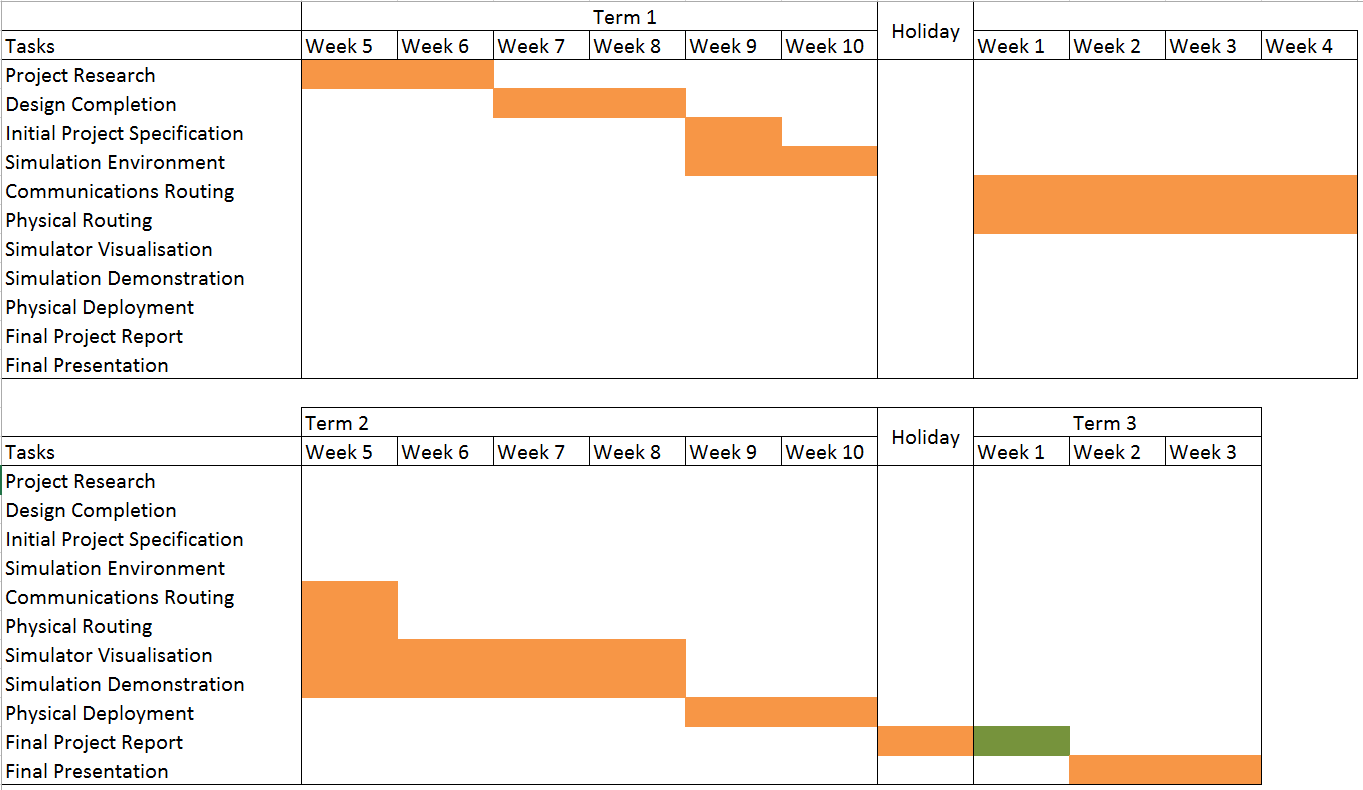
\includegraphics[scale=1,angle=90]{img/progantt.png}
\caption{Gantt chart of project schedule}
\label{gantt}
\end{figure}

\section{Progress Tracking}

\subsection{Meetings}
Regular meetings were scheduled once a week with both the project group and the project supervisor. Meetings with the supervisor consisted of sharing current progress, including any successes and challenges, as well as to seek advice on specific topics of difficulty such as simulation tools, accurately modelling error and routing techniques. Queries were also directed to the supervisor by email outside of meetings where necessary, to handle urgent requests or to check deliverables. 

The general group meetings involved all four members of the group gathering at the Department to discuss progress, assign new tasks as a result of discussions with the supervisor, or re-assign current tasks to improve scheduling. The group also examined the structure of the code, discussed bug fixes and new iterations of code, and corroborated any research findings using collaboration tools, which will be explained in section \ref{colab}. Extra meetings were also scheduled outside of the usual schedule in order to prepare for deadlines, or to coordinate workflow in the event of a task being assigned to more than one member. Certain tasks, such as physical deployment, required members to gather in one location in order to observe and work with the drones in person.

\subsection{Weekly Review}
In accordance with the software methodology chosen for the project, the group also informally discussed the status of the project in accordance with the schedule shown in figure \ref{timeline}, and received an update from each member as to their individual progress. By sharing the current state of each task with other members, it was possible to gauge the overall status of the project and to reassess any tasks which took up an inordinate amount of time. Instances of project review were also reserved for upcoming deadlines to ensure that project deliverables in particular were proceeding as planned. Minutes of meetings were kept in order to keep track of ongoing tasks.

\section{Source Control}
As a software-based project, it is important to ensure proper source control, so that code can be protected and members can be notified of new iterations, and how they differ from previous versions. While the source code itself did not have version numbers explicitly appended to it, Version Control Systems (VCS) were embedded into the collaboration tool used for code, including the ability to add messages which addressed the changes introduced by updated code, and to highlight any potential errors or bug fixes.

\section{Collaboration Tools}
\label{colab}

\subsection{GitHub}
To manage the project material, a git repository was created to ensure consistency amongst the project members' work and safety for the code base. Github, a web-based git repository hosting service, was used to incorporate source code management and distributed revision control to the project code. Each group member had their own repository locally, and branches were also used to ensure that major changes to the code base did not affect the original version of the code. This also allowed each member to avoid overwriting work when committing changes in the same area of code, which would result in merge conflicts. Using Github, the workflow was separated safely and manageably, and previous versions were retained by the repository so that they could not be lost. This also allowed each member of the group to contribute to the same repository without requiring them to be in the same physical space, or constantly exchanging updated code.

\subsection{Google Drive}
Google Drive was also used in order to manage project material, as well as have a backup for the code base and documentation. This is especially useful for project deliverables such as the report and the specification, as each member could collaborate in real-time with one another on the same documents. Google Drive also allowed for access on multiple devices such as phones, tablets and laptops, which was especially convenient for group meetings.

\subsection{Hastebin}
During the development of the project software, Hastebin was occasionally used for individual code snippets, as the UI supports code highlighting and is designed for sharing programming code. Alternatively, a real-time format such as Etherpad could have been used, but Hastebin was chosen for its ease-of-use and due to the fact that individual group members typically worked on separate areas of the same code, so Hastebin was utilised more for checking (incorrect) code than to develop code side-by-side.

\subsection{Facebook}
In order to communicate with other group members, Facebook was used as the primary method of contact. Each group member was already using Facebook, which made it the most common and the easiest way for group members to communicate. Facebook also allows for sharing files, which was found to be more convenient in the case of small files which did not require to be backed up. Facebook became a useful tool for general discussion about the project, including the project schedule and the code, as well as for the dissemination of tasks on-the-fly.

\section{Project Challenges}
At the beginning of the chapter, a summary was given of the main elements which the project was comprised of. In this section, the various challenges which had to be overcome in order to complete the project successfully are analysed. Specifically, areas such as researching, scheduling, organisation and development will be discussed, and how these challenges were dealt with throughout the project. 

\subsection{Planning}
The project was incredibly difficult in terms of the amount of work that had to be done in the limited amount of time available, and so effectively planning how and when each stage of the project would be completed was crucial to the project success. Each task which had to be completed was scheduled using the Gantt chart shown in figure \ref{gantt}, and the group was organised such that each member was aware of their individual tasks and responsibilities, and the timeframe available to them. The Gantt chart provided a good overview of the project activities, as well as being simple to read and understand; it was immediately clear that each member of the group what the current status of the project was, and what had to be completed at what time.

\subsection{Research}
One of the biggest challenges during the project was researching in order to find the proper tools and resources which were available that would be relevant to the project. A comparison of the various simulator libraries which were available was made, in order to find out their complexity, utilisation and functionality, such as ns-3 and OMNet++, and whether or not these libraries were necessary in order to create a drone sensor network. Ultimately, an original simulation was designed and developed by the group, which was influenced by the utilities provided by such libraries, and the use of ns-3 in the early stages of development was helpful to understand the various protocols which would need to be implemented into our own simulator.

\subsection{Development}
Following the planning stages, the project had carefully been broken down into tasks which had to be completed. According to the plan, the simulation would form the basis of physical deployment, in order to simplify the project as a whole and save time. During the development stage, the utmost care had to be taken to ensure that the simulation framework could be effectively transferred over to physical deployment during development. With this in mind, the simulation code was written in such a way that the only remaining factor to consider for physical deployment was the ability to use libraries which would interact with the drone's hardware, such as the ability to takeoff, move, turn, and land. Additionally, creating a simulation which could accurately model real-world communications without the use of network simulator libraries turned out to be a much more difficult task than had originally been scheduled for. The workload was subsequently re-evaluated and scheduled to realistically reflect the amount of time which would be taken, which involved using the time buffer of working over the holidays.

\subsection{Deployment}
When planning for physical deployment, there were several difficulties in terms of working with hardware which was not guaranteed to be suitable for the task. In order to provide autonomy to the drones, it was necessary to attach a Raspberry Pi to the drone, as well as GPS sensors, and then transfer the code base to the Pi in order to control the drone directly. Having no prior experience working with hardware explicitly, the group had to manage to configure the Pi in order to be able to connect and hook into the drone directly through Wi-Fi, and execute the code from the host (or base station). There were also concerns that attaching extra peripherals to the drone would potentially have weighed it down to the point that it would be incapable of sustaining its altitude, which would also affect its autonomous flight plan. The capabilities of the Parrot AR drone in terms of handling heavier payloads had to be researched and tested to confirm the maximum payload weight that it could handle.

\section{Risk Management}
The risks involved with the project are detailed in table \ref{risktable}.

\begin{table}[]
\centering
\caption{List of risks for the project}
\label{risktable}
\begin{tabular}{|l|l|l|}
\hline
\# & Risk Event                                                           & Mitigation                                                                                                                                                               \\ \hline
1  & Team member falls ill during the project                             & \begin{tabular}[c]{@{}l@{}}Reassign tasks where necessary and focus on schedule. Use buffer time\\   if necessary.\end{tabular}                                          \\ \hline
2  & Parrot drones have faulty hardware                                   & \begin{tabular}[c]{@{}l@{}}Reason with Department for replacement hardware and focus on other\\   tasks.\end{tabular}                                                    \\ \hline
3  & Any hardware breaks or is faulty                                     & Same as 2 - replace where necessary or continue without if possible.                                                                                                     \\ \hline
4  & Lack of contribution from a team member                              & \begin{tabular}[c]{@{}l@{}}Attempt to encourage the team member and assist with the task if\\   necessary. If problem persists, consult project supervisor.\end{tabular} \\ \hline
5  & Development turns out to be too difficult technically                & \begin{tabular}[c]{@{}l@{}}Consult project supervisor for advice as to changing the\\   project/project task/how to complete the task in question.\end{tabular}          \\ \hline
6  & Code becomes corrupted or lost due to accident/damage                & Recover backup code from git repository and continue.                                                                                                                    \\ \hline
7  & Simulation environment is too slow to perform as needed              & \begin{tabular}[c]{@{}l@{}}Consider optimisation of simulation as priority over other tasks in\\   order to preserve core functionality\end{tabular}                     \\ \hline
8  & Research for drone sensor networks is limited                        & \begin{tabular}[c]{@{}l@{}}Focus on combinations of alternatives e.g. research on drones,\\   research on sensor networks\end{tabular}                                   \\ \hline
9  & Unable to implement visualisation for the simulation                 & \begin{tabular}[c]{@{}l@{}}Focus on ensuring that other key functionality is achieved/maintained\\   for the simulator and consider as future work\end{tabular}          \\ \hline
10 & Drone gets lost during deployment due to loss of signal/out of range & Liaise with campus security to arrange for retrieval of the drone                                                                                                                                                    \\ \hline
11 & Communications routing is too difficult/time costly to implement     & \begin{tabular}[c]{@{}l@{}}Consider finding and using pre-existing libraries which can be\\   imported to the stimulator\end{tabular}                                    \\ \hline
12 & Physical routing is too difficult/time costly to implement           & \begin{tabular}[c]{@{}l@{}}Consider reverting to core functionality or pre-existing libraries\\   where necessary\end{tabular}                                           \\ \hline
13 & Drones are unable to perform collision detection                     & \begin{tabular}[c]{@{}l@{}}Ensure that drones manage individual, well-separated airspace only\\   and are physically unable to go near each other\end{tabular}           \\ \hline
14 & Physical deployment is not completed on time                         & \begin{tabular}[c]{@{}l@{}}Focus on functionality of the simulator for demo and present\\   theoretical results for real deployment where possible\end{tabular}          \\ \hline
15 & Scheduling is poorly managed and tasks are overestimated timewise    & \begin{tabular}[c]{@{}l@{}}Re-evaluate schedule and use buffer time if necessary. Tasks may also\\   be added or removed where necessary\end{tabular}                    \\ \hline
16 & Demonstration code for simulation is not completed on time           & \begin{tabular}[c]{@{}l@{}}Revert to using example code used to test simulation for demo and\\   physical deployment.\end{tabular}                                       \\ \hline
17 & Use of drones on campus is deemed illegal/unsanctioned               & \begin{tabular}[c]{@{}l@{}}Find open airspace in alternate location which is not monitored/free\\   to use\end{tabular}                                                  \\ \hline
\end{tabular}
\end{table}

\section{Legal, Social, Ethical, and Professional Issues}
The subject of drones has been the focus of much controversy with regards to issues of privacy, invasion of airspace and other unsanctioned uses of UAVs with the ability to, for example, use a camera to take pictures or video. Therefore, a platform for an entire network of drones with a variety of sensors which is open source presents a multitude of possible problems. Furthermore, with the potential to be used as a foundation for military efforts, which form the basis of many current topics of research into drones and sensor networks, there are many implications for potential misuse of the project. As a result, it is necessary to research and discuss the possible methods of unlawful utilisation of drones and drone networks, in order to ensure that the project group is aware of these issues.

\subsection{Legal Issues}
The law is, however, very clear with regards to the use of firearms against UAVs, whether or not the UAV in question was trespassing or invading on private property. In November 2014, a man was fined \$850 in damages for shooting down a neighbour’s drone while it was flying over the neighbour's property, and then refusing to pay any compensation for destroying the drone \cite{colinneagle2015}. The Federal Aviation Administration’s (FAA) definition of a drone as aircraft also means that, technically, shooting a drone could result in a maximum penalty of a 20 year prison sentence. Pursuing legal action in cases such as this is difficult, as it is not illegal to fly a drone in public. 

There are several instances where the definition of misuse of drones has been well established and offenders have been prosecuted. In the very first case of prosecution against unsanctioned drone usage, a security guard was sentenced after repeatedly flying drones over and around Premier league football stadiums, Buckingham Palace and Parliament buildings, where he was fined and banned from flying UAVs \cite{maryannrusson2015}.  In the US, FAA regulations state that drones must not be flown near airports and other areas with manned aircraft, as well as placing a ban on altitudes over 400ft. The Civil Aviation Authority (CAA) in the UK states that for a Small Unmanned Surveillance Aircraft (SUAS) of less than 20 kg, the operation must not endanger anyone or anything, and the aircraft must be within visual line of sight \cite{civilaviationauthority2015}.

For the specific case outlined above, the aircraft being used for surveillance purposes was in violation of the rules of direct line of sight of the aircraft as well as being subjected to tighter restrictions with regard to the minimum distances that you can fly near people or properties that are not authorised. In most instances of prosecution, the owner of the drone would be required to have permission from the CAA to fly their drone in an area that would usually be forbidden access.

There have also been cases of the use of drones in order to smuggle illegal substances into high security areas. Scotland Yard has logged various different drone-related incidents, including complaints about drones being used to ferry drugs into prison \cite{maryannrusson2015}.  It is highly likely that an individual or individuals would be responsible for such use of drones, particularly in violation of multiple laws \cite{civilaviationauthority2015}, as opposed to commercial businesses. However, this implies that open source autopilot software and other similar platforms may be used unlawfully by individuals.

\subsection{Social Issues}
A interesting issue arises where any drone carrying a payload such as a camera has the potential for recording data unlawfully. In one instance, a drone which was found to be hovering over an ATM that seemed to be recording people entering their pin numbers into a cash machine. It can be argued that the drone was not breaking the law by simply recording a public space\cite{maryannrusson2015}. However, it is difficult to prove that the usage of the drone was for the express purpose of obtaining peoples’ pin number, or if this is unlawful to begin with, in the same way that there is no law which expressly forbids someone from looking over the shoulder of an ATM user.

A full-length documentary called Speciesism: The Movie based its foundational discoveries and source of information by using drones to spy on factory farms and record evidence of environmental damage, and went on to feature major global press coverage. In this particular instance, the law with regards to prosecution was unclear, despite the activity being labelled as ‘spying’. This could suggest that such uses of drones, even on potentially private property, may not be possible to prosecute, although this may be unique to incidences of whistleblowing. It will be up to society to determine where the acceptable boundaries of drone usage lie, and how this should be represented in legislation.

\subsection{Ethical Issues}
As discussed in previous sections, engaging in military operations is one of the most prevalent uses for drones, as well as being a popular area for research and development of UAVs. Fortunately, the specifications of consumer-level drones are not of a high enough calibre to warrant usage in the military, which requires state-of-the-art hardware, including weaponry. However, there is an initiative to create small, hand-sized mini drones for soldiers in the US Army, for the purpose of small scale intelligence gathering and reconnaissance, in place of conventional air support \cite{jonfingas2016}. Projects such as this have implications for the usage of drones of all shapes and sizes in military operations, which would suggest that implementations of drone autonomy by hobbyists and businesses may form a basis for research and development in the army.

The use of drones for spying is not only limited to consumers, militaries have also been responsible for deploying drones to spy on civilians in their home country. The Department of Defense in the United States has admitted to using Predator and Reaper military drones in the US since 2006 in order to support domestic civil authorities, which was made public in March 2016 \cite{pentagon2016}. According to the government, these domestic drone flights are stated as not being in violation of any laws, and were being employed in a “very, very minimal way, very seldom”.

\subsection{Professional Issues}
Given that the project is released under an open source license, it is possible that it will be used to perpetrate acts which are illegal or unethical. If there should be an onus on creators to restrict the functionality of their projects, then this has troubling implications in terms of free speech. Additionally, there are many use cases of drones which could be classified as either ethical or unethical depending on intent (reconnaissance for a police drugs raid compared to reconnaissance for a bank heist). 


\chapter{Project Outcome}
	\label{projeval}

\emph{The aim of the project was to create a generic simulation for drone networks which was capable of being extensible to a variety of different UAV hardware, and to prove its effectiveness on the specific use case of the Parrot AR drone by bridging the gap between the simulation and the hardware. This chapter will evaluate the success of the project against the original requirements, including a summary of the results of creating the simulator, the implementation of routing, and the transition to physical deployment. It will also give a summary of how the project scheduling performed compared to the projected schedule, and make suggestions as to how the project could have been extended given a larger timeframe.}

\section{Project Deliverables}

\subsection{Simulator}
One of the biggest challenges to creating the simulator was the decision to migrate from the core functionality provided by ns-3, and instead focus on creating a simulator from the ground up. As a result of research and testing, it was found that ns-3 was too bloated and rigid to create an efficient, general-purpose simulation for drone sensor networks. In place of using a pre-existing library for network simulation, it was decided that the simulator would be built using C++ from first principles. The design and development of the simulator was incredibly successful; despite concerns that the simulator would not be able to accurately reflect a real environment given the size of the workload and the scope of the project, the simulator was capable of initialising a drone sensor network with all of the functionality which was expected of it. Features of the simulator include the ability to create a network environment, instantiate drones (messageable objects), install communications modules on them such that drones (and the base station) can communicate, pass messages based on arbitrary communications protocols, and visualisation of the simulation itself. As the aim was to create a fully functional simulator which could be used to model arbitrary sensor networks, the simulator demonstrates all of the necessary components for the task.
		\subsection{Routing}
In order to ensure that the simulation performed as expected, it had to be capable of effectively modelling communications algorithms and the ability for each node to control its own individual airspace. Additionally, it was necessary for the simulation to be capable of selecting which communications routing protocol to use at runtime, such that the simulation could be generic enough to incorporate any algorithm. This allows the end user to select the optimal algorithm to model the desired environment in terms of energy efficiency, computation time and complexity. For the implementation of physical routing, methods for collision detection and governing airspace were to be defined in the simulator, such that each drone would be able to carry out its own flightplan autonomously, which included calculating a priority in order to resolve potential collisions. Overall, both communications and physical routing were accurately represented in the simulation, and the demonstration simulation reflected the requirements of the design. Physical routing was not as complex as originally intended, as it did not include specific algorithms for pathing, which may have added to the versatility of the simulation.
\subsection{Physical Deployment}
Physical deployment was necessary in order to prove that the simulation could be accurately reflected in the hardware, providing a general use case for the simulation to adapt to. The main tasks for physical deployment included ensuring that the hardware, especially with regards to the peripherals for the drone, could be used correctly, that the simulator could be adapted to the library selected for hooking into the drone, and that the code could be transferred over to the external computer which was attached to the drone. Provided that the simulator accurately modelled real deployment, the assumption was that the code did not have to be re-factored for the sake of deployment. While there were some difficulties with transferring the code over to the Raspberry Pi, the library used for controlling the drone’s physical movements was sufficiently tested, and the drones actually performed according to the simulation which was built to demonstrate a real drone sensor network. Despite concerns about the weight of the drone, the peripherals were sufficiently light, and did not affect the flight of the drone.
	\section{Time Management}
Following the initial planning stages of the project, the group created a Gantt chart in order to schedule the tasks which had to be completed and the amount of time allotted to each task. For example, the design of the simulation environment was to be completed by week 10 of term one. Unfortunately, this schedule was too optimistic and did not reflect the allowances which had to be made for deadlines relating to each group member’s individual work. Each group member had several coursework deadlines scheduled for the end of the first term. As a result, development did not begin until the beginning of the second term; contingency time was allotted to allow for any delays or changes to requirements, and the holiday was able to be used as a buffer for finalisation of the design stage. In order to compensate for lost time, the frequency of group meetings and collaborative coding sessions was increased, and tasks such as communications and physical routing were performed concurrently.
The project was able to progress according to schedule during the second term, as research and development, including the group project report, continued unabated until the final weeks of the term. During this time, the group focused on completing the design for the visualisation of the simulation, the implementation of communications protocols following research, and preparing the drones for physical deployment by testing the hardware and the library which would be used to pipe the simulation framework to the drone itself. The visualisation process was found to be more difficult than expected, and was not fully completed until the beginning of the third term. Nonetheless, the group did not require any extensions for deadlines and successfully delivered the project within time constraints, with minimal changes to requirements and scheduling.
	\section{Requirements Evaluation}
In the specification chapter of the report, the functional and non-functional requirements were carefully established, such that the success of the project could be measured against the utilities which were intended for it.  While it is difficult to measure non-functional requirements in terms of success, most of the core functionality such as sending, listening for, and receiving messages over Wi-Fi or radio can be seen in the simulation. The simulation code was shown to be adaptable to the physical drones for real deployment, and the extensibility of the code as a non-functional requirement can be seen from the results of the simulation demonstration. Additionally, the functional requirements of the project do not provide an exhaustive list of the features contained within the project software, as there are many other features such as simulation timing objects for time-based events which were also included in the simulation. Given that the project is not marketable and that the stakeholders can be identified but not consulted with, it is also difficult to ensure that the project software meets requirements which have not been established by the group. 
Some of the requirements for the projects were not met due to time constraints, and some requirements were adjusted to reflect the status of the project as it progressed. For example, one of the key features which was intended for the project was the ability to implement user input-tasking, where the user could specify a job for the network to carry out. While it is possible to show that the simulation can be extended to the hardware and adapted to any arbitrary task without performing the task explicitly, the project did not progress to a state where a specific demonstration could be shown of the network receiving a task from the user to complete using sensory information and carrying it out. Another functional requirement was the ability of the nodes to move through the environment using pathfinding algorithms chosen at runtime, similarly to communications routing. The drones are capable of moving through the environment by managing their own airspace, but they lack the implementation of more complex, efficient physical routing protocols, and there are no alternatives to the current implementation. However, the lack of these features does not detract from the completeness of the solution, and a result of agile development is simply that the requirements continue to change to reflect the state of the project.
	\section{Future Work}
There are many possible extensions and improvements to the project which could have been implemented, which would have been examined given a larger timescale. In particular, there were many ideas with regards to improving the efficiency of the simulator, improving the API, and adding more communications and physical routing libraries to the system.
The simulation environment is the core of the project software, and one of the biggest problems is the current runtime, which has the potential to be optimised, as discussed in section 6.2. Within the environment, it would be possible to improve the broadcasting function which currently tests the entire list of messageables. This could be improved by attempting to limit the number of messageables to those within the immediate vicinity of the broadcast through segmentation of the environment, which would greatly reduce the overheads involved in checking each messageable object. Another potential extension with regards to the simulator is the upkeep function of the drones, which currently called upkeep one drone at a time, which causes dependencies between drones. This process could be made more efficient by parallelising the upkeep function (in the case of a system that can handle a large amount of threads).
In order to improve the functionality of the simulator, the number of communications routing libraries could also be increased to provide more variety in modelling the environment. The current simulator only supports the Basic messaging protocol as well as routing based on AODV. As a result, the end user who wishes to model the system may find that it is difficult to find the optimal routing protocol for their specific use case. Adding more routing protocols such as DSR would allow for more options when modelling the environment, which would likely allow the user to improve the accuracy of the their network environment by finding the most suitable algorithm. In addition to communications routing, the current simulator code only performs physical routing by allowing each drone to manage its own airspace and avoid collisions. While the basic method of movement and avoiding collision allows for a sensor network to be modelled accurately, it may not reflect the needs of the user and could be further optimised with the use of other existing pathfinding algorithms.
On the note of the end user, it is also important for the simulator to be user-friendly, such that the functions which need to be used to tailor the stimulator to specific hardware are easy to use and understand. Currently, the API is not very readable; it is quite difficult to see which functions are supposed to be used and how. In order to improve the experience for the user, the simulator could be improved by adding prefixes for functions, so that they are more visible, or by adding another level of inheritance to the tree, which would simplify the architecture and make it more secure for the user.
With regards to physical deployment, the project has only implemented a specific use case involving the Parrot AR 2.0 Power Edition drone. In order to aid in the generic nature of the simulation and foster a more complete solution, the simulator could be adapted to more cases using different hardware. In doing so, errors which are specific to the Parrot drone could be highlighted, as well as overcoming issues related to hardware other than the Parrot which have yet to be seen. By attempting deployment on different hardware, the simulator can be shown to be portable to more than one platform and thus capable of being adapted to any arbitrary hardware. While the team envisioned the ability to extend the project software to multiple platforms, this was practically unrealistic given the budget of the project. 

All in all the reference deployment of octoDrone was a great success. The final version of the parrot library was able to take simulator programs and run them on hardware with no changes and simulation files were usable with minimal changes. The quadcopters performed very similarly to our simulations, which simultaneously validates the accuracy of both the simulator and the deployment.

Running distributed applications on the Raspberry Pi was made extremely easy by having the compiled simulation take care of starting and stopping any additional threads it needed to create. This ease of use was such that it piqued the interest of a number of faculty who identified it as being an excellent outreach resource.

The results we managed to achieve also highlight how easy it would be to create a similar implementation for another hardware setup. In theory, it may also be possible to create a simulation which ran on a mixture of simulated and real drones. 

\chapter{Conclusion}
	As a project, the research and development of a generic simulator for implementing drone sensor networks has been incredibly challenging and rewarding. In the previous project evaluation chapter, considerations were made for the success of the project in terms of the components required and how the project was scheduled over the seven month period of the course. This chapter will give an overall outline of the project as a whole, including a summary of the project idea, the design and implementation of project components, the issues which were encountered along the way, and the outcome of the project in its completion. 
The project group, comprised of four people, were able to become acquainted and solidified themselves as a team in order to successfully overcome the tasks and challenges that came with the project. From the very beginning of the project, the team were able to establish a strong working atmosphere and an appreciation for the project concept, and the individual skills that each member would bring to the table in order to see it fulfilled. The project itself came with many hardships; drones sensor networks are a recently emerging field, which meant that it was difficult to find a large amount of material as a topic of research. The idea to create a sensor network with the use of drones in and of itself was a relatively new idea which required many considerations in terms of the feasibility of hardware, software libraries, and the existence of previous solutions to draw inspiration from. The prospect of designing and creating a simulator which could then serve as the framework for the deployment of a physical network of drones was incredibly exciting, and reflected the enthusiasm of each member to work on state-of-the-art technology (and do something really cool with drones). 
The creation of the simulator was originally designed to be based on the pre-existing network simulator ns-3, which is currently the most popular set of libraries for creating a network simulation. As originally laid out in the specification, the project was designed to use ns-3 as the foundation of the network simulator, to aid in the implementation of code which would be transferred to the hardware for deployment. After making the decision to change the basis of the project design by creating a network simulator in C++ from scratch, the group found that it was possible to create a general use simulator which could be adapted to any hardware more readily, and the software components developed into a platform which reflected the objectives of the project more accurately. The design for the simulator environment itself was broken down into its core components: the nodes in the network (drones and base station), the communications modules installed on the nodes, the routing protocols which would be used by the network and the code which would instantiate the environment and execute the simulation. The code for each component was meticulously planned, written, and tested, which was possible due to the modularity of the system, before being migrated into the simulator environment. 
There were many issues with the development of the simulator such as having to implement communications protocols manually, instead of being able to use pre-existing libraries which allow these protocols to be used automatically. While the idea to create a generic simulator from first principles was unique, it presented many challenges in practice, as the level of functionality which could be expected from using a simulator such as ns-3 would not be immediately available or feasible to introduce given the manpower and time scale of the project. However, this decision allowed for the group to create a platform which was simple and easy to manipulate – it contained only the bare necessary functionality for the task at hand, reducing the complexity and computation time significantly. Despite the technical difficulty involved, the group was able to successfully build a platform which could simulate a drone sensor network and output a visualisation of the results.
After the completion of the simulator, the next step was to implement physical deployment by transferring the simulation code over to real hardware. This reflected the objective to move from simulated programs to real hardware whilst avoiding the necessity of rewriting the same software, which is the appeal of the generic stimulator that was created. The physical deployment stage of the project went incredibly smoothly with only minor changes to the original design, such as using Ethernet for internode communication following the realisation that the Raspberry Pis did not have to be attached to the drones specifically. Despite concerns from the group that the hardware would not be compatible with the simulation or each other, alternative solutions were found for any outstanding problems and the project was scheduled such that allowances could be made for any hindrances resulting from hardware issues.
Overall, the project was completed successfully due to careful and concise planning, the enthusiasm and determination of each group member to complete their assigned tasks within their allotted time, and the well-founded management of the project in terms of scheduling and development methodology. The project itself can be said to have made contributions to the world as a combination of multiple fields of research with implications for future development and improved research into the potential of drone and sensor network technology. This includes the decision of the Department to make use of this project as a demonstration to prospective students, with the aims of garnering interest in the pursuit of Computer Science and similar concepts which can be derived from this project.
In final conclusion, the project has been a fantastic learning experience with regards to the development of a large team project over an extended period and the difficulties which are associated with it. The results of the project show that the concept is both possible to implement and expand upon, and that, despite being a relatively new field of research and development, there exist possible applications for future projects. The support and advice from the project supervisor and among the members of the group was critical in reaching the level of success that the project achieved, and it will be exciting for each member of the team to see how similar projects in the field ‘takeoff’ in the future (huehuehuehuehue).


\begin{appendices}
\chapter{API Documentation}
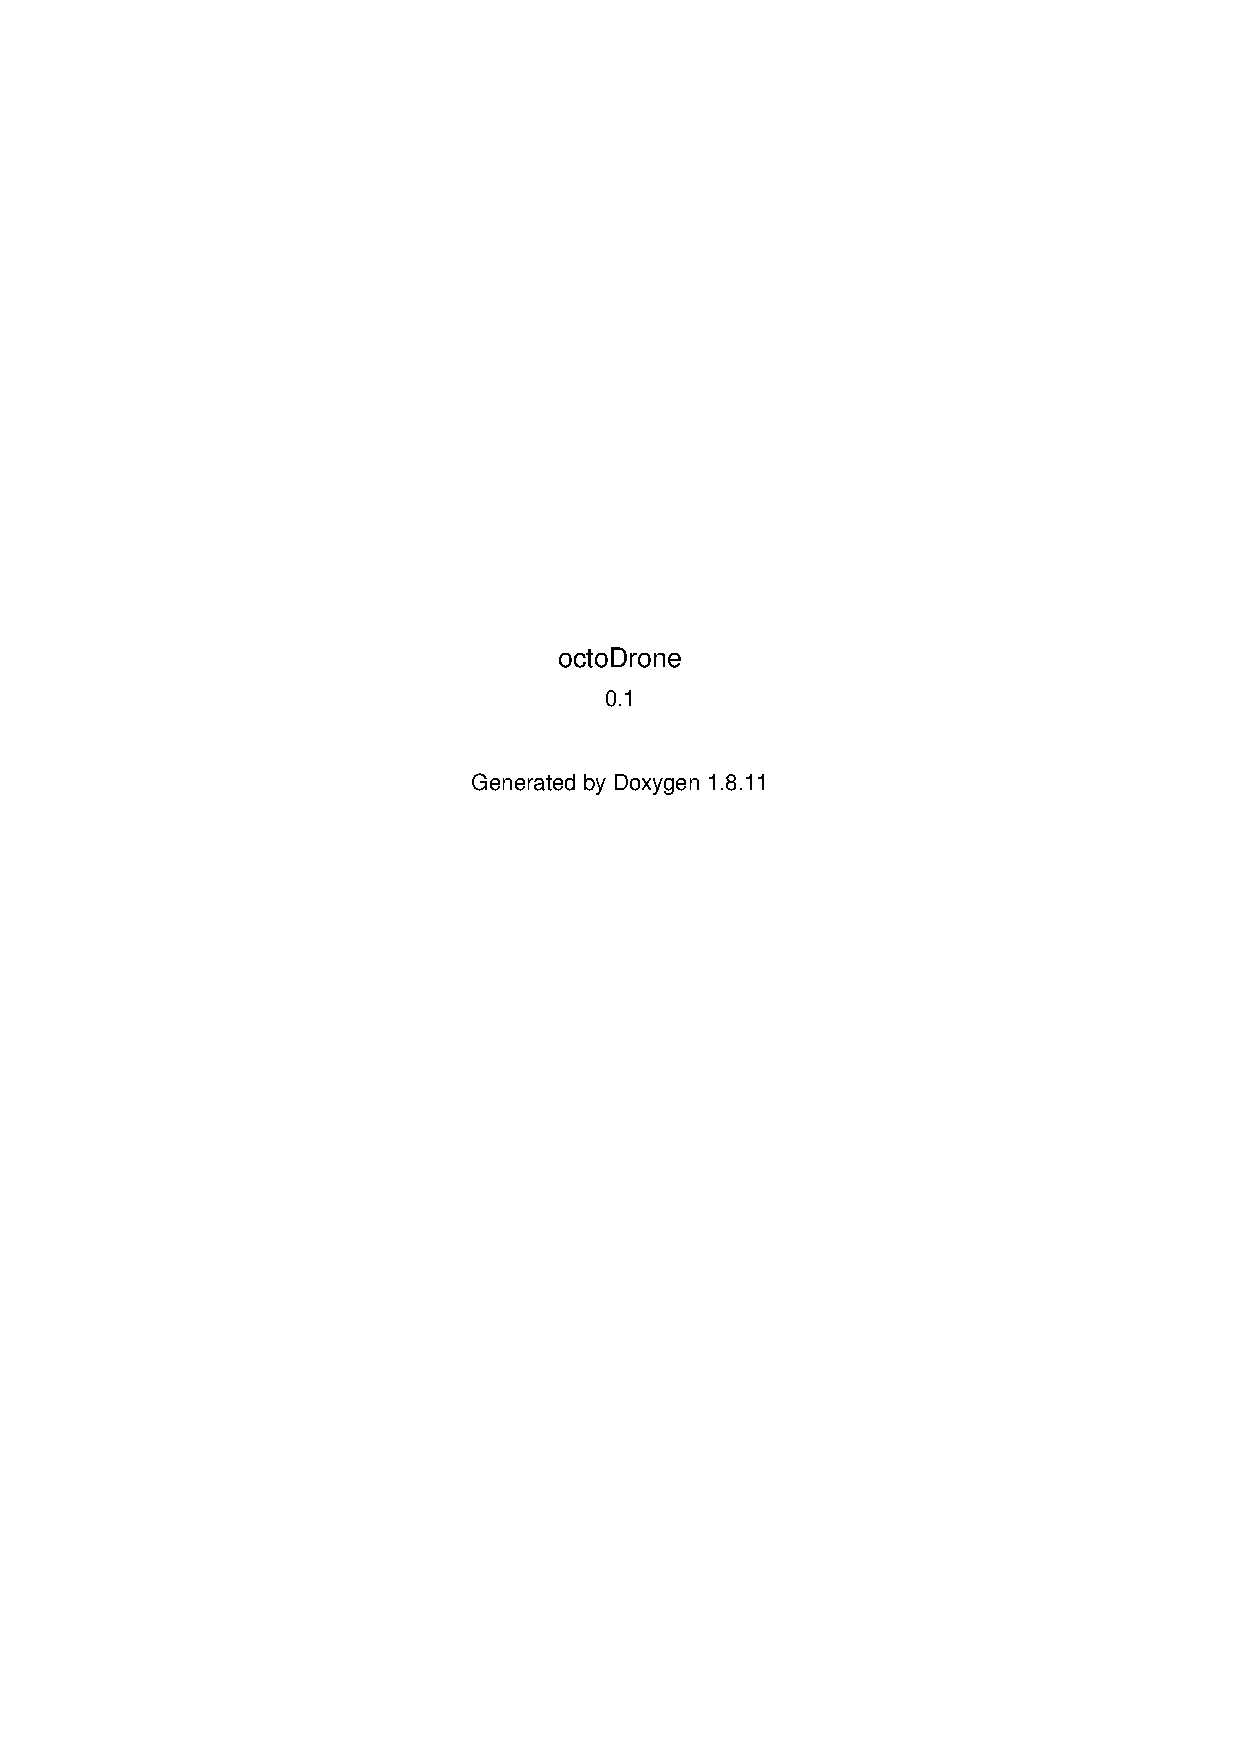
\includepdf[pages={-}]{../documentation/latex/refman.pdf}

\bibliography{biblio}

\end{appendices}

\end{document}
